\documentclass{AIAA_REVTeX41/AIAA}

\usepackage{amsmath}
\usepackage{amssymb}
\usepackage{amsfonts}
\usepackage{pifont}   % http://ctan.org/pkg/pifont
\usepackage{latexsym}
\usepackage{graphicx}
\usepackage{pgf}
\usepackage{tikz}
\usetikzlibrary{arrows}

\usepackage{xcolor}
\usepackage{url}
\usepackage{fancyvrb}
\usepackage{xspace}

\usepackage{alltt}
\usepackage{ifthen}
\usepackage{listings}
\usepackage{placeins}
\usepackage{supertabular}

%% \usepackage{pvs/pvspkg}

%%%  Theorem like environments  %%%

\newtheorem{theorem}{Theorem}[section]
\newtheorem{lemma}[theorem]{Lemma}

%%%  Listings Configuration  %%%

% Sally code listings
%% sally code listings
\lstdefinelanguage{sally}{
  sensitive=true,
  keywords={},
  otherkeywords={% Operators
      not, and, or, =, <, >, <=, >=, =>, +, *, -, /
  },
  keywords=[2]{define-states, define-state-type, define-transition,
               define-transition-system, query},
  keywordstyle=\color{orange},% operator color
  keywordstyle=[2]\color{blue},% keyw color
  numbers=left,
  numberstyle=\scriptsize,
  stepnumber=1,
  numbersep=8pt,
  showstringspaces=false,
  breaklines=true,
  frame=single,
  comment=[l]{;;},
  commentstyle=\color{purple}\ttfamily,
  stringstyle=\color{red}\ttfamily,
  morestring=[b]"
}

\lstnewenvironment{sally}{\lstset{language=sally}}{}

% LIMA code listings
%% lima code listings
\lstdefinelanguage{lima}{
  sensitive=true,
  keywords={},
  otherkeywords={% Operators
      <-, <==, not\_, \&\&., ||., >., <., ==.
  },
  keywords=[2]{atom, channel, cond},% main keyw
  keywords=[3]{readChannel, writeChannel, fullChannel, value, Const},% other keyw
  keywordstyle=\color{black},% operator color
  keywordstyle=[2]\color{blue},% keyw color
  keywordstyle=[3]\color{brown},% other keyw color
  numbers=left,
  numberstyle=\scriptsize,
  stepnumber=1,
  numbersep=8pt,
  showstringspaces=false,
  breaklines=true,
  frame=single,
  comment=[l]{--},
  morecomment=[s]{\{-}{-\}},
  commentstyle=\color{purple}\ttfamily,
  stringstyle=\color{red}\ttfamily,
  morestring=[b]"
}

\lstnewenvironment{lima}{\lstset{language=lima}}{}

% TEXT code listings
%% plaintext code listings
\lstdefinelanguage{plaintext}{
  sensitive=true,
  keywords={},
  keywordstyle=\color{black},% operator color
  numbers=left,
  numberstyle=\scriptsize,
  stepnumber=1,
  numbersep=8pt,
  showstringspaces=false,
  breaklines=true,
  frame=single,
}

\lstnewenvironment{plaintext}{\lstset{language=plaintext}}{}


%% VATSAN BEGIN
\newcommand{\cmark}{\ding{51}}%
\newcommand{\xmark}{\ding{55}}%
\renewcommand{\lstlistingname}{Code Listing}
%% VATSAN END

%% LEE BEGIN
\newcommand{\y}[1]{\texttt{#1}}
\newcommand{\func}[3]{\ensuremath{#1 \, : \, #2 \rightarrow \, #3}}
%% LEE END

%% BEN BEGIN
\newcommand{\OM}{\ensuremath{\mathrm{OM}}}
\newcommand{\OMH}{\ensuremath{\mathrm{OMH}}}
\newcommand{\Id}{\ensuremath{\mathrm{Id}}}
\newcommand{\Msg}{\ensuremath{\mathrm{Msg}}}
%% BEN END


\usepackage{hyperref} %

\newboolean{submission}  %set to true for the submission version
%\setboolean{submission}{false}
\setboolean{submission}{true}
\ifthenelse
{\boolean{submission}}
{ %
  \newcommand{\lee}[1]{ } %
  \newcommand{\ben}[1]{ } %
  \newcommand{\vatsan}[1]{ } %
  \newcommand{\bren}[1]{ } %
  % Put your own TODO macros here and below
} %hide todo
{ %
  \newcommand{\lee}[1]{ {\color{blue}$<$lee: #1$>$} } %
  \newcommand{\ben}[1]{ {\color{purple}$<$ben: #1$>$} } %
  \newcommand{\vatsan}[1]{ {\color{red}$<$vatsan: #1$>$} } %
  \newcommand{\bren}[1]{ {\color{green}$<$bren: #1$>$} } %
  \usepackage[inline]{showlabels} %
}

\begin{document}

\title{A Language for Unified Verification and Implementation for Distributed Avionics}

\author{Benjamin F. Jones\footnote{Senior Research Engineer, 421 SW 6th Ave.} and Lee Pike\footnote{Research Lead}}
\affiliation{Galois, Inc., Portland, Oregon, 97204}
\author{Srivatsan Varadarajan\footnote{Staff Scientist} and Brendan Hall\footnote{Engineer Fellow}} \affiliation{Honeywell Advanced Technology, Golden Valley, Minnesota, 55422}

\begin{abstract}
In designing, verifying, and validating distributed systems today, an engineer is often faced with having to specify a system multiple times. For example, the engineer might specify it once in a model-checker for formal analysis, in an architectural description language for requirements analysis, and in a programming language for testing. By specifying the same system multiple times, there is risk that each specification has different semantics, so that the system tested differs from the one verified, for example. To help solve this problem, we envision an \emph{architectural domain-specific language} (ADSL), or a unified language from which formal models, executable code, and architectural models can be synthesized. To make our problem tractable, we focus on distributed fault-tolerant systems. We present the \emph{\textbf{L}anguage for \textbf{I}ntegrated \textbf{M}odeling and \textbf{A}nalysis} (LIMA), a particular ADSL that we have designed. We describe LIMA and its application to case-studies motivated by avionics design.
\end{abstract}

\maketitle

\lee{%
TODOs:
\begin{itemize}
\item Change pounds to dollars in LIMA examples.
\end{itemize}
}

% ------------------------------------------------------------------------------
\section{Introduction}
\label{sec:problem}

Modern avionic systems continue to grow larger in size and complexity, and
state-of-the-art flight control systems can consist of more than a million lines
of code. Lockheed Martin's F22 Raptor contains approximately 1.7M lines of
code~\cite{dvorak2009nasa} and the next-generation F35 fighter is estimated to
comprise 5.7M lines of code.  This trend is not limited to the military arena;
the software content of the Boeing 787 is estimated at 13 million lines of
code~\cite{judas2011historical}.

Concurrently, advancements in networking technology enable increasingly
distributed systems, and network-centric Integrated Modular Avionics (IMA)
architectures are now the industry norm across all aircraft segments, from large
air transport A380~\cite{itier2007a380} to general
aviation~\cite{ananda2009general}.  This integration of multiple aircraft
functions into IMA architectures offers many benefits. Leveraging common
hardware may enable significant SWaP (size weight and power)
reduction. Standardization on hardware platforms may support the improved
optimization of the system obsolescence management. Finally, the ability to
support more cooperation between traditionally federated aircraft functions may
support greater efficiency and safety. The benefits of such integration are
argued in ~\cite{rushby2000partitioning}.

%% However, the increased functionality and higher levels of integration increases
%% system risks in the form of common-mode influences on the host or networked
%% platform and the interaction state space of the hosted functions. New technology
%% and assurance methods could counter these risks.

Industrial architectures often evolve and are usually based on informal
assumptions. By establishing a formal model of the system, we can uncover many
undocumented assumptions. Once formal models are developed, we have found that
the application of formal methods can systematically uncover edge cases and
erroneous behavior that are not otherwise obvious. For example, in our previous
work developing fault-tolerant
protocols~\cite{dutertre2012model,driscoll2012maximizing}, we found that the
application of model checkers is particularly valuable for uncovering erroneous
edge cases in the protocol logic. In~\cite{dutertre2012model}, we further
demonstrated the ability to leverage the formal models developed during protocol
design to generate system-level test cases.

Formal modeling is typically---but not exclusively---used to reason about
behavior. Architectural modeling helps to document and reason about
non-functional properties. Numerous architectural languages, including
AADL\cite{feiler2006architecture}, EAST-ADL~\cite{debruyne2005east},
SLIM~\cite{bozzano2009compass}, and SYSML~\cite{friedenthal2011practical} have
emerged in the past decade. Analysis tools support the models developed using
architectural modeling notations. These tools support many aspects of system
examination from schedulability~\cite{singhoff2005scheduling} analysis to
failure and propagation analysis (HiHOPs~\cite{papadopoulos2011engineering} and
ADAPT~\cite{liu2009reliability}), and automated fault-tree
generation~\cite{li2011method,joshi2007automatic}.

While introducing formal or architectural modeling into a distributed system
development effort can improve the documentation and quality of the system, it
comes at a high cost. In particular, it means there are three separate artifacts
to maintain and keep consistent: the formal model, the architectural model, and
the actual system implementation. Ensuring their consistency is ad-hoc, as each
language has its own syntax and semantics with no connections between them. At
best, the additional effort required to keep the models consistent outweighs the
benefits of increased assurance. At worst, it provides a false sense of
assurance, where the implementation does not satisfy properties specified in
architectural or formal models.

The central thesis of the research described here is that formal models and
analysis is not cost effective unless those models are integrated into the
software development process so that there is one central view of the system and
the models and analysis are directly connected with the software. Without a
formal link through the system refinement and implementation processes, we risk
the \emph{abstraction gap} where implementation details may impact the
assumptions of the higher level abstract model of the system that has been
formally argued. We call the specification that generates models and
implementations an \emph{architectural domain-specific language} (ADSL). The
user needs only to specify the system in one language, and from that, has
multiple ``views'' onto the system.


 %% composable system analysis and verification is primarily achievable through  \emph{apriori} model synthesis and an iterative, generative approach. We believe that the correct modeling paradigm for distributed systems also needs to support different levels of system abstraction and provide an incremental path of system refinement from the high-level  system models to system implementation.  In addition  to meeting the system assurance needs, we also believe that it is necessary to integrate the levels of abstraction and system refinement to ensure that the assumptions made at one level are suitably accounted for or discharged at the lower or higher level. This accounting is especially important when developing formal models to support the architectural claims and fault-tolerance reasoning of distributed systems. Although formal methods technology has improved, current tools are unable to deal with the lower-level details of system implementation due to simplifying abstractions for tractability of analysis and/or scalability limitations. Instead the formal properties of the system architecture or fault -tolerant protocol services are often formally proved using higher level abstract models.  

%% There are two obvious ways to solving the problem of disconnect between
%% different models. One way is to do post-hoc verification each of the three
%% specifications are refinements (abstractions) of one another. Doing so is a
%% monumental undertaking, requiring specifying the semantics of each language and
%% building verification tools to automatically prove refinement. Even if
%% feasible, it does not solve the problem of having to specify a system in
%% multiple languages.

%% The other approach, which we have taken, is to \emph{generate} formal models,
%% architectural models, and implementations from the same specification. 

\begin{figure}
\begin{center}
\includegraphics[width=1.0\textwidth]{figures/overall_approach}
\caption{ADSL Approach.}
\label{fig:overall_approach}
\end{center}
\end{figure}

Moreover, while the work we describe here focuses on connecting executable software with formal models for verification, it is in service of our vision for an
architectural workbench as shown in Figure~\ref{fig:overall_approach}. We
envision an ADSL from which multiple analyses are available including

\begin{itemize}
\item Synthesizing formal models (e.g., PVS~\cite{SRI:PVS} for interactive theorem-proving or Sally~\cite{sally} for model checking);
\item Synthesizing architectural models (e.g., SysML~\cite{SysML}, AADL~\cite{feiler06aadl-intro,as5506}), hardware models (e.g., Verilog or VHDL), and software models (e.g., Simulink or C/C++);
\item Automate test generation for system testing from ADSL system models;

\item Integrate into assurance case toolsets (e.g.,~\cite{Rushby05anevidential,CruanesHOS13}) to systematically integrate the
  formal system assurance and associated evidence (e.g., artifacts from analysis
  tools, model checkers, theorem provers, and automated test generation) and
  test artifacts. Ideally, these assurance-cases can be constructed in the context of aerospace development
  standards (e.g., DO-178C~\cite{do178c}, DO-254~\cite{do254}, DO-297~\cite{do297}, ARP-4754~\cite{arp4754}, ARP-4761~\cite{arp4761}).

%% \item Generate low-level implementation, domain-specific languages from system specification  specifically for hardware (e.g., BSV, Chisel, Confluence~\cite{nikhil:bluespec,bachrach2012chisel,TomHawkins:Confluence}) and software (e.g., Ivory, ATOM, Copilot, Scade, Simulink~\cite{ivory:dsl,pike-rv,atom:dsl,esterel:scade,matlab:simulink}) with a path to scoping of directed individual hardware and software component V\&V coverage.
\end{itemize}

\noindent
We have not completed this full integrated vision, but our ADSL makes significant advances toward it. In particular, we address the difficult aspect, which is developing a succinct language for specifying distributed systems with sufficient fidelity to synthesize implementations as well as formal models for verification.

Such a vision touches upon a wide range of research, which we highlight in
Section~\ref{sec:current}, particularly focusing on architectural description
languages and formal analysis tools, our current focus. Earlier, we have
described our language as an \emph{domain-specific} language; the domain we
focus on here are fault-tolerant distributed systems commonly found in aerospace
systems. Toward that end, we outline the concepts that a language specialized
for this domain should imbue. For example, such a language must be able to succinctly allow designers to specify and reason about different fault models, message-passing constructs, and real-time constraints. We describe these concepts in Section~\ref{sec:towards-adsl}. The concepts drive the design and implementation of the ADSL itself, described in Section~\ref{sec:adsl}. There we introduce the prototype ADSL we have built, which we call LIMA, standing for ``\textbf{L}anguage for \textbf{I}ntegrated \textbf{M}odeling and \textbf{A}nalysis''. We also describe our compilation strategy to both C code and to the input language of Sally, a state-of-the-art model-checker~\cite{sally} that LIMA targets. In particular, the translation to Sally is particularly novel, as we describe an efficient encoding of time, distributed communication, and faults that is amenable to decidable formal analysis. To demonstrate the effectiveness of LIMA, we present case-studies drawn from aerospace systems in Section~\ref{sec:case-studies} that we model in the LIMA and generate executable source code and formal models. These case-studies highlight a unique design feature of the LIMA: it is an \emph{embedded} domain-specific language (EDSL), meaning that it is hosted in a general-purpose programming language. The EDSL approach is common in the programming languages community; we show how it can be used to build powerful new modeling abstractions without introducing new primitives.
 Finally, we present conclusions and future work in Section~\ref{sec:future-work}.




% ------------------------------------------------------------------------------

\section{Related Work}
\label{sec:current}

In this section, we overview related tools and approaches for modeling and verifying systems. We focus on architectural modeling languages and formal verification specialized for distributed systems, particularly noting their strengths and weaknesses with respect to specifying and reasoning about architecture, behavior, and faults in a unified way.

\subsection{Architectural Modeling Languages}\label{ssec:modeling}
The Architecture Analysis and Design Language (AADL) was one of the first system architecture languages, evolving out of the META-H~\cite{binns2001formalizing} language developed by Honeywell as part of the DARPA DASADA program. Since its conception, AADL has matured significantly and is now standardized by the Society  of Automotive Engineers (SAE) under AS5506~\cite{as5506}. AADL is primarily intended to be a system integration language, allowing generation  of an integrated  model that address  different aspects of the system to be captured.  At the core,  AADL provides a common notation that supports the   specification of  both  logical and physical aspects  of the system architecture. The core language is component-based. The physical aspects of the system may be specified utilizing a extensible palette of hardware component primitives, such as processor, device,  and system components, which may be interconnected with bus components and access connections. 
 The logical notation of AADL is  also component-based.  AADL provides a number of software/logical model primitive abstractions, such as system, process, thread, subprograms, that allow for logical model specification. In the logical model, components are interconnected using data and event port connections. The core of AADL also allows for the association between the logical and physical models to be specified by binding property annotations to the model.

Through a flexible annex mechanism, the  core  AADL language can be extended
with user-defined syntax. Different aspects of the system can be specified using
dedicated annexes.  Of specific interest are the behavior
and error annexes, and the emerging constraint and hybrid annexes.  The behavior
annex allows for discrete behavior to be specified  using a finite state machine
annotation that can be associated with the logical abstraction components. This
behavior may be fused with the platform behavior of the AADL core to implement a
full system simulation~\cite{dissaux2014smart}.  Similarly, the error annex
annotations allow probabilistic component  error models and state machines to be
associated with each component.  Error flow and error propagation  annotations
are also possible  to describe cross component error propagations and
influences.

Using such annotations, model-based safety analyses are possible, with the annotated AADL model used as the basis for for fault-tree generation~\cite{joshi2007automatic}. Recent annex developments include the requirements annex~\cite{blouin2011defining} that allows a systematic refinement and  association of requirements with AADL model elements, and the hybrid annex, that intends to  extend AADL to address continuous system
models, and a constraint annex that allows for constraints and structural assertions to be defined and executed  within the AADL modeling framework.

The System-Level Integrated Modeling (SLIM) is a simpler variant of the ADDL. It
has been developed as part of the COMPASS project~\cite{bozzano2009compass,gong2013automated}. The intent of SLIM is to generate
formal architecture language that can be used as the basis of architectural
analyses using formal methods. To this end, SLIM is much simpler than AADL,
excluding some of the elaborate AADL features for  hierarchical abstraction and
interface complexity management. SLIM also excludes some of the tasking and
dispatch semantics of the underlying platform execution model. Therefore,
logical abstractions, such as a periodic thread dispatch, need to be explicitly
modeled  using the SLIM behavioral language.  However, in SLIM,  behavioral and
error modeling is integrated into the core model. Using a mechanism called model
extension, SLIM allows these annotations to be integrated into a  formal
transition system model that can be used as the bases for formal analysis. Thus, SLIM supports an integrated view of nominal and error behavioral models.  This differs significantly from the AADL approach, where there is little  formal cross-annex linkage or semantics.

MILS-AADL, a derivative of AADL, is also under development as part of the DMILS-project\cite{dmils}.
This work is also targeting synthesis towards back end formal verification tooling using BIP~\cite{basu2011rigorous}. The D-MILS project additionally targets implementation platforms based on TTEthernet.

The Robot Architecture Definition Language (RADL)~\cite{li2014radl} is a minimalist  AADL targeted towards the design of multi-rate distributed systems. It is under development by SRI. Similar to SLIM, RADL is simpler than AADL, and forgoes the more elaborate features interface and property specification.  RADL is also targeted towards a quasi-synchronous system architectural pattern, in which all nodes asynchronously execute  tasks and exchange messages at defined periodic intervals~\cite{radl}. The RADL framework also incorporates an automatic build system, \emph{Radler}, which synthesizes glue code and platform binding code. At the time of writing, RADL does not incorporate fault  modeling.

SysML~\cite{SysML} extends UML to address the needs of system engineering. It has been standardized under the OMG. SysML comprises a very rich palate of notations that can be utilized to specify system structure and behaviors.  The notation is extendable, making it very adaptable to different modeling needs. Given a disciplined model-based system engineering approach, SysML can be used to capture the functional, logical and physical aspects of architecture, as demonstrated by Pearce and Friedenthal~\cite{pearce2013practical}.

Through dedicated profiles, SysML notation can be extended.  For example, via a Modelica profile~\cite{paredis20105}, SysML can be used to model continuous systems. An automated translation is also available between Modelica and SysML.  Similar translations are also under development for VHDL-AMS~\cite{verries2013case}. SysML-AADL profiles have also been developed to support formal platform modeling~\cite{behjati2011extending,cofer2012compositional}. SysML supports relating requirements across all of the modeling elements.

Due to the flexibility of the notation, SysML can therefore be used to capture many aspects of a system archiecture using a common notation. SysML further provides a requirements framework to allow requirements to be refined via associates to modeling  blocks, providing a similar capability to the AADL requirements annex discussed above.

Recent work addresses fault modeling within SysML~\cite{pearce2013practical}, allowing SysML models to be annotated with failure modes, although this work is less mature than the AADL error annex.

The SCADE-System~\cite{scade} defines an IMA modeling profile that provides a framework to define functional, logical and physical platform models within SysML. The tool also provides an extensive framework to generate Interface Control Documents (ICD) from integrated models. The tool additionally provides code generation to configured commercial partitioned operating systems and network configuration tables from the system model.  The SCADE\_System tool is fully integrated with the SCADE
Suite, hence lower-level system behaviour can be specified in SCADE but remains linked to the higher level architecture.  Such properties make this variant of SysML and interesting synthesis target for ADSL.

Matlab's Simulink~\cite{simulink} is  one of the most widely used
model-based-design notations. It provides a very rich
simulation capability that allows for behavioural exploration. However, the
Simulink notation lacks many of the features required for architecturally
centric design; for example, the separation of logical and platform designs and
the associated bindings is missing. The core language also lacks formal
semantics, and is defined with reference to the behavior of the simulator. The
tooling also offers limited provisions for structured design and design
factoring, which may also limit its applicability to true architectural
modeling.    That said, many production systems have been developed using Simulink, and additional tools have been developed to broaden the
applicability of Simulink.   One such tool is HIPHOPS~\cite{papadopoulos2011engineering}, that allows for fault and error annotations to be added to the Simulink models, and provides a framework to use the model as the basis of Failure Mode and Effects Analysis (FMEA) and system fault-tree analysis and generation.
 
%% Here we briefly summarize other modeling languages for distributed systems. Our
%% main goal in this work is to fill a gap that exists in languages for specifying
%% fault-tolerant, real-time distributed systems in avionics that can be compiled
%% to software, hardware, and formal verification and testing systems.

%% There are two dimensions on which to consider other tools: (1) with respect to
%% their tooling and (2) with respect to the languages and primitives for
%% specifying distributed systems. With respect to the first point, we are aware of
%% few tools or specification languages that can support verification, code
%% generation, and simulation. With respect to the second point, however, there are
%% many languages available.


\subsection{Distributed System Modeling Languages}
A variety of formal modeling and verification languages and tools have been
developed specifically targeting distributed systems.  Hoare's
\emph{Communicating Sequential Processes} (CSP) is one of the original and most
influential distributed system process calculi~\cite{csp}. CSP-based tools such as
CSP$_M$~\cite{cspm}, JCSP~\cite{jcsp}, FSPJ~\cite{fspj}, and
CSP$++$~\cite{cspplus} have been developed and are summarized and compared in a
recent report~\cite{csp-masters}. Notably, CSP$++$ is a relatively recent tool
that includes code generation capabilities to generate C$++$ implementing the
semantics of a specified system. Because it uses the same input language as
other tools, such as FDR, a CSP-based model-checker~\cite{fdr}, specified
systems can be model-checked. However, application code must be written by-hand
and spliced in. This ability is unsound insofar as application code can break
invariants of the concurrency model. However, a tool like CSP$++$ takes
promising steps in the direction of the research we present.

That said, the basic semantics do not typically handle the aspects of distributed systems
with which we are concerned. For example, there are no built-in notions of
faults or timed behavior. Perhaps more significantly, CSP has a dynamic
model of a process, in which a process can be composed to form new processes. A
more static notion of processes may be appropriate in our domain. Indeed, note
the following, when trying to formalize a very simple fault-tolerant protocol in
various CSP-based tools:

\begin{quote}
As with the previous examples, our goal in this project is to use our three
translation techniques on each example. The Byzantine Agreement Protocol,
however, proved to be far more complex than the other examples. So complex, in
fact, that the various shortcomings of each technique proved too substantial to
achieve translation~\cite{csp-masters}.
\end{quote}
\noindent
We present a specification of Byzantine Agreement in Section~\ref{ssec:synchronous-om1} within our ADSL.

\subsection{General-Purpose Formal Verification Tools}
General-purpose formal verification tools have been applied extensively to the specification and verification of fault-tolerant distributed systems.

Model checkers such as the \emph{Symbolic Analysis Laboratory}
(SAL)~\cite{SRI:SAL}, SMV~\cite{nusmv}, and the \emph{Temporal Logic of
  Assertions} (TLA)'s model-checker~\cite{tla} have been used to specify and
verify both software and hardware distributed systems and
protocols~\cite{Rushby-OM1,pike-afm,brown_pike_06,pike_johnson:emsoft,amazon-tla,Dutertre-Sorea-2004}. Model-checking
is one of the most successful verification approaches for distributed systems,
as the technology is ``push-button'' and model-checkers have become
exponentially more powerful as a function over time. Tools such as SAL and the recently-developed infinite-state verification tool \emph{Ivy}~\cite{ivy} allow users to supply invariants to scale verification. Still, most approaches to
model-checking require ad-hoc abstractions and by-hand models. One goal of our
ADSL workbench is automatic translation to model-checkers, creating sound
abstractions for the user automatically.

Work in controller synthesis, usually from temporal logic specifications, has
recently been applied to fault-tolerant algorithms~\cite{BloemBJ16}. In this
work, a simple self-stabilization protocol is synthesized from an LTL
specification using Boolean satisfiability. The approach uses a \emph{counter-example-guided inductive
  synthesis} approach~\cite{Solar} to improve scalability.

Another synthesis approach is followed by Liu~\emph{et al.} with their
\emph{DistAlgo} language and tool~\cite{distalgo,distalgo2}. \emph{DistAlgo}
provides constructs for specifying distributed fault-tolerant algorithms
embedded in a programming language, like Python. While specifications are terse,
it can generate fairly efficient code, both in code size and execution
efficiency~\cite{distalgo2}.

Theorem-proving, in contrast to model-checking, is largely manual but quite
powerful. In particular, PVS~\cite{pvs} has a long history of being used to
specify and verify distributed systems~\cite{unified,fmcad07}. Like with
model-checking, abstractions are usually ad-hoc and specifications are done
by-hand. There is usually no formal correspondence with an implementation.


% ------------------------------------------------------------------------------

\section{ADSL Desiderata}
\label{sec:towards-adsl}
We first motivate the need for another architectural description language, then we present the fundamental concepts necessary for such a language. We focus on three concepts: clock models, channel \& buffer models, and fault models.

\subsection{Why Another ADL?}

With the numerous architectural description languages (ADLs) and accompanying
tools available (see Section~\ref{ssec:modeling}), we must ask is
is, \emph{"Why another ADL?"}.
We are focused on the correct specification and synthesis of distributed systems
and the formal verification and validation of distributed system protocols.  A
key research goal is to provide a specification framework that encompasses a
suitable level of abstraction to allow for the efficient behavioral
specification of distributed fault-tolerant protocols.  Additionally, we desire
for protocol specifications to exist within the larger context of the system
architecture and anticipated fault models.

Currently, AADL is one of the most mature ADLs, yet, in our work to date we have
found that expressing the details such of protocols with AADL is non-trivial,
with certain aspects not yet possible. such as behaviours that are not
compatible with the underlying AADL dispatch semantics.

%% Although AADL may evolve
%% to capture the required semantics, the pace of change that can be accommodated
%% with standardized languagesis another concern.  Only now, two years after the
%% research completed, are the some of the changes identified by the
%% AFCS~\cite{afcs} research are getting addressed by the AADL working
%% committee. Rather, than pace our research with such timescales, we feel that
%% there may be greater benefit in identifying the needs through our targeting of
%% AADL as an implementation language.

A second goal is integrating the models of faults and behavior.  Once again,
this is an area where current ADLs are lacking. For example, in
AADL, the integration of the behavioral and error annexes is not mature, and
hence cross-annex formal semantics and linkages are not defined.  In addition,
although the LIMA language (see Section~\ref{ssec:modeling}) incorporates provisions
for integrated specification, the level of abstraction is more
cumbersome than it should be.  This is another area where our
synthesis strategy to an intermediate ADL may be beneficial; For example, using
our approach, we may be able to efficiently synthesize LIMA models for formal
analyses, where such models may too expensive to develop by hand.

The final intent is to link the formal assurance argument within the ADSL work
flow. Once again, this is an area where the current ADLs continue to develop;
the recent work with AADL and RESOLUTE~\cite{gacek2014resolute} look
promising.

In summary, there exist no ADLs that allow the efficient
specification and refinement of system models and protocol specification. Our
hope is that it will be more efficient and lighteweight. That said, where formal
semantics exist for intermediate ADLs, our ADSL can target them.


%% However, rather than be limited by the current capabilities, our
%% intent is that ADSL can link to what works and where necessary develop new
%% capabilities to address areas of identified need.


%% Finally, given the ADSL's functional host langauge (see
%% Section~\ref{sec:adsl}), we further anticipate great benefits as we leverage
%% test generation frameworks such as QuickCheck~\cite{monadic} to the
%% architectural specification, especially if such generation can be aligned with
%% the formal fault model.

%% \subsection{ADSL Approach}
%% The core of the technical approach is that we are able to synthesize both formal
%% models and implementation models directly from the ADSL specification in
%% our ADSL workbench. In order for the ADSL to be useful, it has to be expressive
%% enough with sufficient variety of primitives to cover a breadth of models
%% supporting varying networks, architectures, and systems as covered by the case
%% studies described in Section~\ref{sec:case-studies}. The ADSL must also be rich
%% enough to describe in sufficient depth each case study to go from high level
%% architecture models (e.g., AADL) to all implementation level details and models.

%% \lee{This needs to be fleshed out}

%% Currently in our research, we have restricted ourselves to primarily focusing on
%% developing SAL~\cite{SRI:SAL} formal models and AADL architectural models as targets
%% to be synthesized from our ADSL specification.  Our strategy is two fold.

%% First, we take a \emph{bottom-up} approach of describing some basic elements and
%% building blocks that must be captured in our ADSL
%% (Section~\ref{subsec:ADSL_Elements}). The idea is that
%% then we will have to flesh out enough of these basic building blocks and build
%% layers of abstractions from them, composing them systematically (potentially
%% hierarchically) and constructing larger models of the systems of interest based
%% on our case studies from them.

%% Second, we also take a \emph{top-down} approach of describing the targets for
%% the three case studies in Sections~\ref{subsec:ADSL_CaseStudy_1}
%% and~\ref{subsec:ADSL_CaseStudy_3} that help us drill down further and narrow
%% some of the ADSL primitives that definitely must be developed.

%% With both the approaches described above, we have gained valuable insights
%% and intend to incorporate the lessons learned into the ADSL and corresponding
%% synthesis framework within the ADSL workbench. At the time of writing,
%% we do not yet have exact and full ADSL specifications with appropriate
%% abstractions nor have we completed all of the actual
%% synthesis for targets for the given case studies (though we have the synthesis
%% framework itself) . We are still in the process of researching the right levels
%% of abstractions in the ADSL framework and the costs/benefits of synthesis with
%% respect to the scalability of the formal models so synthesized in terms of its
%% ability to prove different properties of interest and efficiency of synthesis to
%% implementation models.

%% So at the time of this report we simply outline the progress we've made thus far
%% and also describe some of thoughts that should feed into the development of the
%% ADSL specifications and ADSL development in years II and III.


\subsection{ADSL Concepts}
\label{subsec:ADSL_Elements}

The three fundamental concepts we present are clocks, channels \& buffers, and faults to describe real-time distributed systems. We describe each in turn.

As we describe the following, we present the concepts based on the notion of an \emph{atom}. An atom is a hierarchical state-machine. An atom can represent a node in a distributed system, but we also allow for the existence of a \emph{sub-atom}, that is a sub-component of a node. Atoms allow us to decompose specifications. We call a sub-atom's encompassing atom the sub-atom's \emph{parent}.

\subsubsection{Clock Model}
\label{subsubsec:clock_model}

\begin{figure}[h!]
\centering
\caption{Clocked Atom Model}
 \includegraphics[width=0.75\textwidth]{figures/clocked_atom.png} 
\label{fig:clock_atom_model}
\end{figure}

In modeling distributed systems, we must often assign clocks to atoms to measure its notion of the passage of time. The notion of clocked nodes are \emph{periodic} processes or tasks.  A clocked atom is defined by a tuple of three parameters as shown in Figure~\ref{fig:clock_atom_model}:
\begin{itemize}
\item {\it startup} which indicates the duration of time elapsed from time $0$ when the clock starts ticking away i.e. initialized \emph{start up delay} for the clock. Note that this startup can span multiple periods potentially. $startup \geq 0$
\item {\it phase} is the \emph{offset} within the period when the task/process is executed periodically. $0 \leq phase < period$
\item {\it period} is the periodicity of the task i.e. inverse of the frequency of the task.
\end{itemize}

All \emph{derived} clocked atoms or \emph{sub-atoms} from parent have synchronous clock with respect to the parent clock. This means, as shown in figure \ref{fig:sync_clock_atom_model}, the $startup$ of the sub-atoms are identical to parent and their clocks are initialized identical to the parent. A shown in the figure both $atom1$ and $atom2$ derived from $atom$ have identical $startup$ parameter. Also the \emph{derived atoms's phases are additive} Thus $atom1$ has an effective phase $phase+phase1$ from start of period and $atom2$ has an effective phase $phase+phase2$ from the start of the period. Also derived atoms period are harmonic with respect to the parent and at equal or slower rate. For example in the figure $period1 = period$ while $period2 = 2 \times period$. Thus atom and sub-atom relationships can be used to model synchronous system whereby all distributed system nodes which are synchronous with each other can be modeled as sub-atoms with clocks under a single parent atom with a ``notional'' clock for the whole system. Similarly ARINC~653~\cite{arinc653} partitions or tasks within a singe node can be modeled as sub-atoms with a single parent atom.


\begin{figure}[h!]
\centering
\caption{Synchronous Derived Atom Clock Model}
 \includegraphics[width=0.75\textwidth]{figures/sync_clocked_atom.png}
\label{fig:sync_clock_atom_model}
\end{figure}

All derived sub-atoms have a synchronous clock with respect to the parent clock. That is, as shown in Figure~\ref{fig:sync_clock_atom_model}, the $startup$ of the sub-atoms are identical to their parent atom, and their clocks are initialized identically to the parent. A shown in the figure, both $atom1$ and $atom2$ derived from $atom$ have an identical $startup$ parameter. Also, the derived atoms's phases are additive. Thus, $atom1$ has an effective phase $phase+phase1$ from start of period and $atom2$ has an effective phase $phase+phase2$ from the start of the period. Finally, derived atom periods are harmonic with respect to the parent and at an equal or slower rate. For example, in the figure, $period1 = period$, while $period2 = 2 \times period$. Thus, atom and sub-atom relationships can be used to model synchronous systems whereby all distributed system nodes which are synchronous with each other can be modeled as sub-atoms with clocks under a single parent atom with a ``notional'' clock for the whole system. Similarly, ARINC 653~\cite{arinc653} partitions or tasks within a singe node can be modeled as sub-atoms with a single parent atom.

\begin{figure}[h!]
\centering
\caption{Asynchronous Peer-to-Peer Atom Clock Model}
 \includegraphics[width=0.75\textwidth]{figures/async_clocked_atom.png}
\label{fig:async_clock_atom_model}
\end{figure}

On the other hand, as shown in Figure~\ref{fig:async_clock_atom_model}, two peer clocked atoms at the top level are considered \emph{asynchronous} with each other. As shown in the figure, their individual $startup$, $phase$, and $period$ for their respective clocks have no relationship with each other.

During verification, it can be useful to allow startup times, periods, and phases to be nondeterministic (without violating the constraints above) to verify timing properties about the system under abstract constraints. For example, one might state timing constraints and verify that the system implements time-triggered behavior~\cite{fmcad07}. During C simulation, however, these timing values must take on constant values.


\subsubsection{Channel \& Buffer Model}
\label{subsubsec:channel_buffer_model}


System designers typically have to contend with managing resource constraints across networked systems. There are two high level resources they need to balance: (i) platform resources like CPU utilization (time) and memory (space) vs (ii) network resources like bandwidth/link usage manifesting as transport/channel delay (time) and network card memory/channel buffers (space). Since both platform and network resources along both time and space dimensions are all finite, optimizing along just one of those resources and/or dimension at the cost of the other is not a viable option. Correct characterization of computation time, communication time (channels delay) and associated buffers (memory at platform or network) at every node is a critical element of the ADSL as it lays the foundation for accurate modeling of platform and network resources in the system.  We show the time and space attributes of network resources in terms of channel and buffer models in Figure~\ref{fig:channel_buffer}. 

A channel is modeled as \emph{unidirectional} flow of message $M$ from a transmitter Node $T$ to multiple receiver Nodes $R_1,R_2,...,R_n$ with corresponding channel delays $D_1,D_2,...,D_n$. Channel delays are all different because there may be different transport paths from transmitter to the different receivers. Channel delays are a function of the size of message $M$, the network bandwidth/link rates, the propagation time (wire length) and the number of intermediate relays between transmitter and the receiver. Thus a message transmitted on to the channel at time $T_1$ from Node $T$ is received at each of the receiver from the channel at times $T_1+D_1, T_1+D_2, T_1+D_3,...,T_1+D_n$ respectively. Note that \emph{unicast}, \emph{multicast} and \emph{broadcast} all supported with this model of channel.

Also note that as shown in the Figure~\ref{fig:channel_buffer}, there is string of \emph{producing} processes and \emph{consuming} processes in the model and this must correctly identified in-order and in-sequence to get the modeling of the buffer (e.g. overflow or size) correct and this is described next. For example, in Node $T$, there is some platform application that is producing a message (possibly from a computation process) and this produced message is stored in the channel buffer (network card memory). The network card in Node $T$ subsequently reads from its own memory (channel buffer) and produces (transmits) the message on to the channel. 

The process is then reversed at the receiver. The receiver network card consumes the message from the channel and stores the message locally into own channel buffer (network card memory). Then either the network card reads from its channel buffer and pushes the message to consuming platform process OR the consuming platform process reads from the channel buffer and then finally processes the message as it sees fit (possibly sent to a computation process).

Since Produce/Transmission at $T$ and Consume/Reception(s) at $R$ can be triggered by “independent” clocked atoms (described in section \ref{subsubsec:clock_model}) at $T$ and $R(s)$. So buffer model is critical to manage the differences in rates and timing between production and consumption. Once the processes are correctly modeled as stated above, then we identify two types of channel buffers at either the transmitter or at the receivers:
\begin{itemize}
\item \emph{Queuing}: First-in-First-Out (FIFO) Order i.e. messages are taken out of the queue in the order in which data was produced into it.  The maximum size of the queue is also specified upfront $k$. If messages are not consumed at fast enough rate compared to rate at which message are produced into the buffer and once the queue is already filled with   “k” messages yet to be consumed, then produced message(s) are dropped. 

\item \emph{Sampling}: New message produced overwrites old message if not consumed.

\end{itemize}


\begin{figure}
\begin{center}
\includegraphics[width=0.8\textwidth]{figures/channel_buffer.png}
\caption{Channel and Buffer Models}
\label{fig:channel_buffer}
\end{center}
\end{figure}

\subsubsection{Fault Model}

The ability to model and specify fault models is a  significant capability
of the proposed ADSL. Faults can occur at different levels of abstraction, and an ADSL should have the capability of specifying and reasoning about faults at the different levels as well as mapping between them.

In particular, we distinguish between local and global faults.
Following the taxonomy of Avizienis~\emph{et~al.}~\cite{taxonomy},
we refer to faults that occur locally in any component, such as a node or channel, as being modeled as \emph{local faults}. Some examples of
local faults are:
\begin{itemize}
  \item Omission (message loss)
  \item Commission (babbling)
  \item Untimely (late, early, sequence violation etc.)
  \item Invalid value (semantic, syntactic,..)
  \item Invalid protocol behavior (e.g., failure of fault handling of detection,
protection etc).
\end{itemize}

On the other hand, \emph{global faults} are based on relationships between
two or more components (i.e., nodes or channels) at the system level. Examples of system
faults include \emph{symmetric} and \emph{asymmetric} transmission faults~\cite{Tha88:RDSS}. Global faults
may be dependent on the expected of degree of consensus~\cite{lynch}, which in itself is
tied to the application's sensitiveness to disagreements, independence assumptions, or degree of maliciousness (e.g. assumptions on how coordinated two or more nodes can be in triggering failures). Global faults based on relationships between two or more components and can cause interactive consistency (consensus violations) and byzantine issues at the system level.


\begin{figure}
\begin{center}
\includegraphics[width=0.8\textwidth]{figures/fault_propagation.pdf}
\caption{Fault Propagation}
\label{fig:fault_propagation}
\end{center}
\end{figure}

Finally, we wish to also characterize fault
propagation through the networked system, originating in some component and
propagating from one component to another, as shown in the bottom of
Figure~\ref{fig:fault_propagation}. Faults introduced/propagated from upstream
components transform to other faults based on protection mechanisms built
into
each component (e.g., a commission fault transforms into an omission fault
if a
bandwidth check is implemented as protection mechanism in a component)~\cite{theory}.

To illustrate this in a concrete example, refer to a cyclic redundant check
(CRC) protection behavior illustrated at the top of
Figure~\ref{fig:fault_propagation}. Nominally in a fault-free operation,
$Node_1$ adds a CRC to a message when it transmits over the channel, and
when
$Node_2$ receives the message, it does a CRC check by comparing the re-computed
CRC
with the frame check sequence (FCS). If the check fails, the message is dropped,
and if the check
passes, then the FCS is stripped and the message is forwarded. Note that
fault-free
(nominal behavior) of a CRC check at the receiver is that (i) a good message
is
never dropped incorrectly, (ii) a bad (corrupt) message is dropped with high
probability, and (iii) there is also a small finite probability that a bad
message escapes detection and drop (e.g. based on efficacy of CRC 32 etc)~\cite{crc}.

Value Fault~1 in Figure~\ref{fig:fault_propagation} introduced in the node
either at the indicated point or introduced upstream before that point and
propagated until that point will also continue to propagate downstream and
CRC
offers no protection. This is because the FCS is added on an already corrupted
message. Value Fault~2 introduced in the channel will be protected by CRC
(modulo the CRC's efficacy). Further Value Fault~2 will transform to Omissive Fault downstream due the CRC protection. 
Value Fault~3 introduced in $Node_2$ at that
point will propagate downstream as it is after CRC protection.

The idea then is to capture a fault transformation function in every
component
node/link based on behavior fault-protection schemes available at that component;
e.g., a value fault transforms to an omissive fault for CRC protection. 
These will be
specified in a static manner at every component. This way, both horizontal
propagation of faults (CRC example) and vertical propagation of faults
(e.g., self-checking hardware) can be modeled as component embedded
in another
component) can be captured in ADSL framework.




% ------------------------------------------------------------------------------

\section{LIMA: an ADSL Implementation}
\label{sec:adsl}

%% In modeling fault-tolerant distributed systems, we want to be able to
%% address behavior and properties which depend on timing and communication
%% delay. For example, in the TTA startup protocol~\cite{Dutertre-Sorea-2004},
%% timing and transmission delays during synchronization are critical to
%% analyzing fault tolerance. 

%% Our language, \textbf{LIMA} addresses the three main
%% concerns implicit in this idea: fault modeling, specification of distributed
%% systems, and specification and analysis of systems with real-time constraints.

%We start by looking at the main syntactic elements of the language.
LIMA, which stands for ``\textbf{L}anguage for \textbf{I}ntegrated
\textbf{M}odeling and \textbf{A}nalysis'', is a domain specific
language embedded in the functional language Haskell~\cite{haskell98}. Its
implementation makes heavy use of Haskell as the host language for
expressing macros, enabling parametrization, and the handling of
parsing and low-level compilation.

The approach is an example of the embedded domain-specific language (EDSL) approach, which allows type-safe, Turing-complete compile time programming, and has been used in a number of domains, from embedded software~\cite{ivory-15} to runtime monitoring~\cite{pike-rv} to GPU programming~\cite{Chakravarty:2011:AHA:1926354.1926358}. Indeed, LIMA is built on the Atom EDSL~\cite{atom}. Atom was originally designed for bare metal embedded systems programming that supported concurrency without requiring a real-time operating system. The state machine language, in which the computation of individual nodes is expressed, is within the language of Atom~\footnote{Atom documentation can be found at \url{http://hackage.haskell.org/package/atom}.}.

We first present LIMA's syntax in Section~\ref{ssec:lima-syntax}. Then we describe code synthesis in LIMA in Section~\ref{ssec:code}. Formal model synthesis is presented in~\ref{ssec:formal-model-synth}. Finally, we briefly describe visualization tools associated with LIMA models in Section~\ref{ssec:lima-visualization}.

LIMA is designed to implement the desiderata described in Section~\ref{sec:towards-adsl}. However, as a initial implementation, some desiderata have not been fully implemented. We describe its current status below.

%%%%%%%%%%%%%%%%%%%%%%%%%%%%%%%%%%%%%%%%%%%%%%%%%%%%%%%%%%%%%%%%%%%%%%%%%%%%%%%%

\subsection{Syntax}\label{ssec:lima-syntax}


Our goal here is to introduce the LIMA. We are not, however, providing a comprehensive overview of the language, but we present the major elements. In particular, we elide the portion
of the language focused on building state machines internal to an
individual node or process. The node-local state machine language is described in the Atom itself.

We first introduce the basic building blocks of LIMA for modeling communicating state machines. Then we describe the LIMA fault model.

\subsubsection{Specifying Communicating State Machines}\label{sec:syntax}

There are
two main syntactic elements: \emph{atoms} and \emph{channels}.

\begin{itemize}
\item \emph{Channel}: Channels are typed and unidirectional. A channel is
declared in a monadic context as follows:
\begin{lima}
(tx, rx) <- channel name ini
\end{lima}
\noindent
creating two endpoints, \y{tx} and \y{rx}, that are user-defined
variables. These variables are ``handles'' for the channel that can be emitted
or read on, respectively. The types of \y{tx} and \y{rx} must agree in all
contexts. \y{name} is a plain text name for the channel, used to connect the
syntax at this level to the formal model and C code syntax after generation.
Finally, \y{ini} is an initial value for the contents of the channel.

% BFJ: include these or not?
%
% Channels also subsume the declaration of environmental signals. A clock tick
% and an interrupt signal are declared, respectively as follows:
% \begin{alltt}
% rx <- clock 5

% rx <- signal name (1`ms`)
% \end{alltt}
% \noindent

% The first declaration creates a clock that signals every 5 ticks,
% transmitted on a channel. The ``tick'' is a unit of time which is
% configurable in the backend.  Only a \y{rx} portion of the channel is
% created, since the clock is which creates the signal is outside of the
% model (and is created by the backend).  Likewise, a \y{signal} creates a
% named signal, together with a deadline for servicing the signal. The
% name denotes some external variable, such as a register.

\item \emph{Atom}: An atom defines a state machine that atomically
handles an incoming message, updates state, and possibly emits new
messages on other channels. An atom may, optionally, do this on a
specified period and phase.
%
\begin{lima}
myAtom rx tx = atom "myAtom" $ do
  v <- readChannel rx
  s <== value v
  writeChannel tx (Const 42)
\end{lima}
%
\noindent
The code above defines an atom named \y{``myAtom''} that handles
a message received on a channel with a receive handle \y{rx}. A channel
must be \emph{dereferenced} to extract a value from it. In the
declaration above, the dereferenced value, \y{v}, is stored into some
shared-state variable \y{s} whose scope exceeds the current definition,
and the value 42 is emitted on a channel with transmit handler \y{tx}. Here,
we use the term ``handler'' to mean a function that takes an incoming message
and returns an action to perform, usually doing some computation and sending
out new messages.

Atom are hierarchical, i.e.\ an atom may contain other atoms and thus define a
hierarchy of global state variables and sub-atoms. All atoms declared
within a parent atom have access to the shared state of the parent. For example,

\begin{lima}
parent = atom "parent" $ do
  s <- int "sVar" 0
  atom "myAtom0" $ do
    ...
  atom "myAtom1" $ do
    ...
\end{lima}
\noindent
declares an atom named \y{``parent''} that contains a shared state
variable named \y{``s''} initialized to zero. It also contains two
handlers, \y{myAtom0} and \y{myAtom1}.
\end{itemize}

A typical pattern in the language is to declare a top-level atom as a
container for one or more channels and one or more sub-atoms which communicate
over the channels.

\begin{lima}
parent = atom "parent" $ do
  (tx, rx) <- channel "myChannel" 0
  s <- int "sVar" 0

  atom "myAtom0" $ do
    writeChannel tx 5

  atom "myAtom1" $ do
    cond $ fullChannel rx
    v <- readChannel rx
    s <== v
\end{lima}

\noindent
In this example, \y{myAtom0} sends the message \y{5} to \y{myAtom1} who stores
it directly in the shared variable \y{s}. The syntax \y{cond \$ \ldots}
declares a guard that must be true in order for the atomic action in that
block to be taken.

Finally, in addition to the hierarchical structure of shared state, the atom
to sub-atom relationship extends to guards. The execution of a sub-atom is
predicated not only on its guard condition, but also that of its parent, its
parent's parent, etc.

\subsubsection{Specifying Faults}

Here we  explain how we account for fault models in LIMA, leaving the
technical details of how faults are encoded in the formal model to Section~\ref{ssec:fault-models}. Part of the philosophy behind our ADSL is that node
behavior and fault behavior should be separate in order to make reasoning
more modular. It is not a surprise then that the number and type of faults to
be included in the model is not specified along with the node behavior.
Instead, it is specified only in the compiler configuration.

Currently there are three options for fault model in LIMA:

\begin{itemize}
    \item \textbf{No Faults}. All nodes in the system perform as designed and channels
        deliver all messages on time.
    \item \textbf{Fixed Faults}. A mapping from node name to fault type is given,
        alowing the designer to specify statically the nature of faults to be
        considered.
    \item \textbf{Hybrid Fault Model}. The designer specifies numerical weights for
        each of three types of fault: manifest, symmetric, and byzantine. In
        this mode, the model-checker will explore all possible configurations
        of nodes with different faults as long as the weighted sum of
        node-fault combinations doesn't exceed a given total.
\end{itemize}
%
The last option is the most powerful form of reasoning about faults in the
system that LIMA offers. It generalizes the well-known results of Park and
Thambidari~\cite{Tha88:RDSS} and Lincoln and Rushby~\cite{Lincoln-Rushby}.

The fault model is decomposed from LIMA's atom's and channel model to specify communicating state machines. This is because we need to be able to synthesize executing code from the system; the fault model is used only within a formal verification. Thus, the fault model is presented as additional configuration data about the environment. The configuration is passed to the Sally model-checker compiler.


%%%%%%%%%%%%%%%%%%%%%%%%%%%%%%%%%%%%%%%%%%%%%%%%%%%%%%%%%%%%%%%%%%%%%%%%%%%%%%%%

%% \subsection{Backend Compilation Strategy}
%% \label{ssec:compilation-strategy}

\subsection{Code Synthesis}\label{ssec:code}

In the LIMA framework we can translate specifications into executable
implementations by generating C code. The code generator is optimized for
embedded targets, those running without a real-time operating system. Although,
the code also compiles and runs on POSIX systems as well.

At a high level, the code generator collects all the atomic actions given in
a specification and translates them into C functions which are executed on a
fixed, deterministic schedule. The schedule is determined by a scheduler which
takes into account each atom's preferred period and phase. The scheduler also
computes the number of basic expressions present in each atomic action so that
the real-time per tick can be calibrated. In section
\ref{ssec:formal-model-synth} we discuss synthesizing formal models from LIMA
specifications. By contrast, in the formal models the schedule is left
non-deterministic but fixed in each system trace.

\begin{figure}
\begin{lima}
ex4 :: Atom ()
ex4 = atom "ex4" $ do
  x <- int64 "x" 0
  y <- int64 "y" 0

  clocked 2 0 $ atom "atomX" $ do
    incr x
    decr y

  clocked 5 3 $ atom "atomY" $ do
    incr y

  assert "y not positive" (value y <=. 0)
\end{lima}
\caption{Example specification with two periodic atoms}
\label{fig:code-gen-example}
\end{figure}

As an example, consider the specification in Figure
\ref{fig:code-gen-example}. Two shared variables are declared and two periodic
atoms update their values. The code generator produces a C structure
representing the global system state; in this case it consists of two
integers. The fields of the struct are nested in several name spaces designed
to keep local variables in different atoms from conflicting. The two atomic
actions are translated into ``rules''; C functions that are called by a main
driver function. Figure \ref{fig:code-gen-rule} shows the rule generated for
\y{atomX}. Finally, the rule functions are driven by a scheduling function
that is responsible for maintaining a global clock value, executing the rules
in the correct order and time, and executing assertion statements. This is
shown in Figure \ref{fig:code-gen-scheduler}.

\begin{figure}
    \begin{lstlisting}[language=C,
                       numbers=left,
                       numberstyle=\scriptsize,
                       stepnumber=1,
                       numbersep=8pt,
                       showstringspaces=false,
                       breaklines=true,
                       frame=single]
struct {  /* state */
  struct {  /* ex4 */
    struct {  /* ex4 */
      int64_t x;
      int64_t y;
    } ex4;
  } ex4;
} state;
    \end{lstlisting}
    \caption{Global state structure in the generated C code}
    \label{fig:code-gen-state-struct}
\end{figure}


\begin{figure}
    \begin{lstlisting}[language=C,
                       numbers=left,
                       numberstyle=\scriptsize,
                       stepnumber=1,
                       numbersep=8pt,
                       showstringspaces=false,
                       breaklines=true,
                       frame=single]
/* Rule { 0, ex4.ex4.atomX } */
static void __r0() {
  bool __0 = true;
  int64_t __1 = state.ex4.ex4.x;
  int64_t __2 = 1LL;
  int64_t __3 = __1 + __2;
  int64_t __4 = state.ex4.ex4.y;
  int64_t __5 = __4 - __2;
  state.ex4.ex4.x = __3;
  state.ex4.ex4.y = __5;
}
    \end{lstlisting}
    \caption{Translated rule for \y{atomX}}
    \label{fig:code-gen-rule}
\end{figure}

\begin{figure}
    \begin{lstlisting}[language=C,
                       numbers=left,
                       numberstyle=\scriptsize,
                       stepnumber=1,
                       numbersep=8pt,
                       showstringspaces=false,
                       breaklines=true,
                       frame=single]
void ex4()
{
  {
    static uint8_t __scheduling_clock = 0;
    if (__scheduling_clock == 0) {
      __assertion_checks(); __r0();  /* Rule { 0, ex4.ex4.atomX } */
      __scheduling_clock = 1;
    }
    else {
      __scheduling_clock = __scheduling_clock - 1;
    }
  }
  {
    static uint8_t __scheduling_clock = 3;
    if (__scheduling_clock == 0) {
      __assertion_checks(); __r1();  /* Rule { 1, ex4.ex4.atomY } */
      __scheduling_clock = 4;
    }
    else {
      __scheduling_clock = __scheduling_clock - 1;
    }
  }
  __global_clock = __global_clock + 1;
}
    \end{lstlisting}
    \caption{Generated scheduler function}
    \label{fig:code-gen-scheduler}
\end{figure}

The final piece of C code generation is a user supplied \y{main} function
which should repeatedly call the generated scheduler function. This is
typically a tight loop with a call to the scheduler followed by a delay
statement that should be calibrated for the platform and desired amount of
real-time per system tick.

Auto-generated code like that shown in Figure \ref{fig:code-gen-scheduler} is only
meant to be machine readable, not human readable. One should think of this code as
an intermediate representation on the way to native machine code. It can be used
by human designers for debugging purposes if really needed, but the LIMA language and
complilation tool chain is setup to avoid exposing users to these low level details.

Execution of the generated code can be very useful in the design and debugging
of systems in LIMA. To that end LIMA provides several debugging features that
can be used along with forward execution in order to examine the state of the
system as it evolves over time. A special primitive function called \y{probe}
allows the user to setup a hook which monitors the value of any expression at
any point of a specification. These probes can be printed out as part of the
system execution by calling another special function \y{printProbe}. In Figure
\ref{fig:code-gen-probes}, the running example has been modified to include
probes on certain runtime expressions and to print the values of those
expressions out on every tick. The output generated during the example's
execution is shown in Figure \ref{fig:code-gen-print-probes}.

\begin{figure}
\begin{lima}
ex4 :: Atom ()
ex4 = atom "ex4" $ do
  x <- int64 "x" 0
  y <- int64 "y" 0

  clocked 2 0 $ atom "atomX" $ do
    incr x
    decr y
    probe "x + y" (value x + value y)

  clocked 5 3 $ atom "atomY" $ do
    incr y
    probe "y" (value y)

  assert "y not positive" (value y <=. 0)
  mapM_ printProbe =<< probes
\end{lima}
\caption{Probing the values of two runtime expressions}
\label{fig:code-gen-probes}
\end{figure}

\begin{figure}
\begin{plaintext}
y: -1
x + y: 0
y: -1
x + y: 0
y: -2
x + y: 0
y: -1
x + y: 1
y: -2
x + y: 1
y: -2
x + y: 1
y: -3
\end{plaintext}
\caption{Printing probes during execution}
\label{fig:code-gen-print-probes}
\end{figure}

% \begin{figure}
% \begin{lstlisting}[language=plaintext]
% Period  Phase  Exprs  Rule
% ------  -----  -----  ----
%      2      0      6  Rule { 0, ex4.ex4.atomX }
%      5      3      4  Rule { 1, ex4.ex4.atomY }
%                -----
%                   10
% \end{lstlisting}
% \caption{Scheduler output}
% \label{fig:code-gen-scheduler-output}
% \end{figure}


\subsection{Formal Model Synthesis}\label{ssec:formal-model-synth}

In this section, we describe our approach for mapping the syntax and semantics
of LIMA to a formal transition system model suitable for model checking.
(Translation to C code is relatively straightforward and we omit its
description here.) One of the main arrows of Figure~\ref{fig:overall_approach}
points from ADSL to ``formal models''.  In the following sections we describe
concretely how a system specified in LIMA can be translated into a
model-checker, while preserving important semantic constraints.

\emph{Efficiently} translating to a model-checking system without
relying on ad-hoc, problem-specific abstractions to make the translation
feasible is an open research problem that we focus on herein.

Let us return to our handler example from the previous section. Execution of
the handler updates the state of the system and so in our translation it is
represented by a transition relation. In Sally, transition relations are
specified by predicates over the ``current'' and ``next'' states of the
system. These are denoted by prefixing state variables with the namespaces
``state'' and ``next''. The transition represented by the handler becomes in
Sally a predicate. Syntatically it is an S-expression with boolean value that
references the state variables.

\begin{figure}[ht]
\centering
\begin{lima}
handler rx tx = atom "someHandler" $ do
  let v = readChannel rx
  s <== v
  writeChannel tx (Const 42)
\end{lima}
\caption{Handler in the ADSL}
\label{fig:adsl-handler}
\end{figure}
%
%
\begin{figure}
\centering
\begin{sally}
;; someHndler:
(and msg_pending(state.cal, state.rx)
   (= next.s           msg_read(state.cal, state.rx))
   (= next.cal         msg_send(state.cal, state.tx, 42))
   (= next.other_var1  state.other_var1)
   (= next.other_var2  state.other_var2)
   ... )
\end{sally}
\caption{Handler as part of a formal model}
\label{fig:sally-handler}
\end{figure}

The variable \y{cal} in Figure~\ref{fig:sally-handler} is a state variable
referencing the ``calendar'', a data structure which keeps track of the times
that future events will take place. Sending a message is
implemented by adding a (future) time, channel identifier, and message content
to the calendar. At the proper time, a transition is enabled for the receiver
to act upon the message. This mechanism is described in more detail below. In
the Sally transition relation, the notations \texttt{msg\_pending(\ldots)},
\texttt{msg\_read(\ldots)}, and \texttt{msg\_send(\ldots)} are short hand for more
complicated expressions:

\begin{itemize}
    \item \texttt{msg\_pending} is a boolean expression that checks whether
        there is a message available for delivery at the current time.
    \item \texttt{msg\_read} returns a message value from the appropriate
        entry in the calendar.
    \item \texttt{msg\_send(\ldots)} is an calendar-valued expression which
        computes the new value of the calendar, typically involving the
        overwrite of a calendar entry with the message contents and the overwrite
        of the entry's delivery time with the current time plus the configured
        message delay.
\end{itemize}

Various kinds of systems with real-time constraints can be implemented
on top of the calendar automata framework. In LIMA, two main
constructs are used to express features such as periodic execution
and aperiod timeouts. First, there is a primitive function \y{clocked},
which takes a concrete period value (in ticks) and either a concrete
phase value (between 0 and the period), or a special value that
indicates phase should be indeterminate. In this context, indeterminate
phase means that phase of execution is non-deterministic, but fixed
within each system trace. This allows us to explore phase-dependent properties
in real-time systems such as the Automatic Airbreak System case study presented in
\ref{airbuscs}.

Second, there is another primitive function \y{writeChannelWithDelay} which,
like \y{writeChannel}, sends a message over a channel, but with a specified
delay added to the delivery time. This feature can be used to program
reset-able, aperiodic timeouts. For example, in the following specification, a
node sets itself a timeout of 100 ticks, after which it sets a flag.

\begin{lima}
timeout = atom "timeout" $ do
  flag <- bool "flag" False
  (tx, rx) <- channel "self_loop" False
  writeChannelWithDelay 100 tx true

  atom "on_wake" $ do
    cond $ fullChannel rx
    flag <== true
\end{lima}

In this example, the relationship between the
outer atom and the inner atom is key. The \y{flag} and \y{channel} are shared between
the two atoms (being in scope for both of them), but the ``on\_wake'' atom's
execution is predicated on the guard of both itself, and it's parent. Since
the parent has no guard in this case we can think of ``timeout'' and
``on\_wake'' as two different nodes communicating over the ``self\_loop''
channel.

% TODO: describe how faults are specified, but not how they are encoded, leaving
% that for later subsection.



%%%%%%%%%%%%%%%%%%%%%%%%%%%%%%%%%%%%%%%%%%%%%%%%%%%%%%%%%%%%%%%%%%%%%%%%%%%%%%%%

\subsubsection{Calendar Automata}\label{ssec:calendar}

Real-time system verification in general-purpose model-checkers
requires an explicit formalism of real-time progression. Trying to
encode real-time clocks directly is difficult; in particular, one
must avoid Zeno's paradox in which no progress is made because state
transitions simply update real-valued variables by an infinite
sequence of decreasing amounts whose sum is finite. To avoid this
problem, Dutetre and Sorea developed \emph{calendar
automata}~\cite{Dutertre-Sorea-2004}, which is itself inspired by
event calendars used in discrete-event simulation. Rather than
encoding ``how much time has passed since the last event'', it
encodes ``how far into the future is the next scheduled event'',
and a real-valued variable representing the current time is updated
to the next event time.

Define a set of \emph{events} $e_0, e_1, \ldots, e_n \in E$. For now, we
do not define events; intuitively, an event is a set of state variables
(shortly, we will associate events with messages sent in a distributed
system). When an event is \emph{enabled}, the transitions over events
are enabled; otherwise, the variables stutter (maintain the same value).

An \emph{event calendar} $\{ (e_0, t_0), (e_1, t_1), \ldots, (e_n, t_n)
\}$ is a set of ordered pairs $(e_i, t_i)$ called \emph{calendar events}
where $e_i \in E$ is an event and $t_i \in \mathbb{R}$ is a
\emph{timeout}, the time at which the event is scheduled. We denote
element $(e_i, t_i)$ of an event calendar by $c_i$.

Let $cal$ be an event calendar and $c_i, c_j \in cal$ be calendar
events. Define an ordering on calendar events such that $c_i \leq c_j$
iff $t_i \leq t_j$, and $\min(cal) = \{ c_i | \forall c_j \in cal, \,
c_i \leq c_j  \}$ are the minimum elements of $cal$.

Let a transition system $\mathcal{M} = (S, I, \rightarrow)$, be a set of
states $S$, a set of initial states $I \subseteq S$, and a transition
relation $\rightarrow \subseteq S \times S$. We implicitly assume a set
of state variables such that each state $\sigma \in S$ is a total
function that maps state variables to values. We sometimes prime a state
to denote that it satisfies the transition relation: $\sigma \rightarrow
\sigma'$. We also sometimes use a variable assignment notation to
describe what state variables are specifically updated: e.g., $\sigma' =
\sigma[v := v+1]$.

We distinguish two special state variables in a transition system: (1)
$now \in \mathbb{R}$ denotes the current time in the state, and (2)
$cal$ is an event calendar.

The following laws must hold of a transition system $\mathcal{M}$
implementing a calendar automaton:

\begin{enumerate}

\item \label{cal:a} Time is initialized to be less than or equal to
every calendar timeout: $\forall \sigma \in I$, $\forall (e_i, t_i) \in
\sigma(cal)$, $\sigma(now) \leq t_i$.

\item \label{cal:c} In all states, if the current time is strictly less
than every calendar event, then the only enabled transition is a
\emph{time progress} update: $\forall \sigma \in S$, $\forall (e_i, t_i)
\in \sigma(cal)$, if $\sigma(now) < t_i$, then $\forall \sigma'$ such
that $\sigma \rightarrow \sigma'$, $\sigma' = \sigma[now := \min(cal)]$.

\item \label{cal:d} In all states, if the current time equals a timeout,
then the only transitions enabled are calendar event updates associated
with the timeout: $\forall \sigma \in S$, $\exists (e_i, t_i) \in
\sigma(cal)$ such that $\sigma(now) = t_i$ implies $\forall \sigma'$
such that $\sigma \rightarrow \sigma'$, $\sigma'(now) = \sigma(now)$,
$\sigma'(c_j) = \sigma(c_j)$ for all $c_j \in \sigma(cal)$ such that
$c_j \neq c_i$ (recalling that by convention, $c_i = (e_i, t_i)$), and
$c_i \notin \sigma'(cal)$.

\end{enumerate}

From the definitions, it follows that in every state, the timeouts are
never in the past, and that time is monotonic:

\begin{lemma}[Future timeouts]\label{lem:ft} $\forall \sigma \in S$,
$(e_i, t_i) \in \sigma(cal)$, $\sigma(now) \leq t_i$.  \end{lemma}

\begin{lemma}[Monotonic time] $\forall \sigma, \sigma' \in S$, if
$\sigma \rightarrow \sigma'$, then $\sigma'(now) \geq \sigma(now)$.
\end{lemma}

Proofs of these two lemmas are straightforward and omitted.

In a distributed system, it is convenient to distinguish global actions
and local actions. Global actions are principally interprocess
communication, while local actions are those carried out by each process
to update its local state and produce new messages to broadcast. While
both global and local actions can both be modeled as events in a
calendar automata, doing so is generally overkill and complicates the
model. From the global perspective, individual processes can update
their local state atomically.

Again, following Dutetre and Sorea, we associate calendar events with
channels in a distributed system~\cite{Dutertre-Sorea-2004}. Specializing calendars to
message passing does not lose generality since all external
communication from an individual process can be abstracted as message
passing. Furthermore, fault models can be abstracted to act over
channels rather than processes~\cite{abstractions}. The calendar
introduces real-time constraints on when processes send and receive
messages.

Assume processes are indexed from a finite set $\Id$. A \emph{channel}
from process $i$ to $j$ is an ordered pair $(i,j)$. Fix a set of
messages $\Msg$. Given a channel and a timeout, let $send$ be a relation
on messages sent on a channel at a given time: $$send \subseteq \Id
\times \Id \times \mathbb{R} \times \Msg$$ So $send(i, j, t, m)$ holds
iff $i$ sends to $j$ message $m$ at time $t$. Likewise, let $$recv
\subseteq \Id \times \Id \times \mathbb{R} \times \Msg$$ be a relation
on messages received on a channel at a time, so that $recv(i, j, t, m)$
holds iff the message $m$ received by $j$ from $i$ at time $t$.

In the absence of faults, we require that messages received were
previously sent and not previously received: if $(i, j, t, m) \in recv$,
then $\exists t'$ such that $(i, j, t', m) \in recv$ where $t' < t$, and
$\neg\exists t''$ such that $t' < t'' < t$ and $(i, j, t'', m) = (i, j,
t, m)$. (We address faults in Section~\ref{ssec:fault-models}.)

Then an event calendar for sending and receiving messages on channels is
the union of the $send$ and $recv$ relations.

The event of receiving a message initiates a process to update its local
transition system and generate additional messages to send. When the
process is updating its local transition system, the event calendar is
paused. That is, updating an event $(i, j, t, m) \in recv$ also includes
updating $j$'s transition system.


%%%%%%%%%%%%%%%%%%%%%%%%%%%%%%%%%%%%%%%%%%%%%%%%%%%%%%%%%%%%%%%%%%%%%%%%%%%%%%%%

\subsubsection{System Properties}
\label{ssec:lima-properties}

In order to specify safety properties of a system in our ADSL, we've chosen to
use the synchronous observer pattern~\cite{Rushby-2012}. The synchronous
observer is a module that is composed with a target system synchronously. Its
job is to monitor the state variables of the system and raise a flag when
safety properties are violated. This idea is a popular alternative to
specifying properties in a special language (usually a temporal logic like
LTL) that has the advantage of being written in the same language and
environment as the system. Additionally, writing a synchronous observer is
second nature to the systems engineers; it is essentially like adding a runtime
check to a program.

Using observers allows us to sidestep the integration and expression of
temporal logic in our ADSL. Instead, the programmer adds an observer to her
system as a top-level monitor along with annotations that indicate which state
variables are to be observed.  From this we automatically generate a
corresponding observer module as well as the theorems and lemmas that the
model checker expects.

Our experiments with a few specific distributed fault-tolerant systems suggest
that using synchronous observers in place of LTL properties introduces very
little overhead during verification.


%%%%%%%%%%%%%%%%%%%%%%%%%%%%%%%%%%%%%%%%%%%%%%%%%%%%%%%%%%%%%%%%%%%%%%%%%%%%%%%%

\subsubsection{Fault Models}\label{ssec:fault-models}

The typical approach to modeling faults is to add new state variables to each process representing its fault state. Then a node chooses actions based on its fault state. As a simple example, we might define a node that sends a good message if it is non-faulty and a bad message otherwise. In pseudo-code using guarded commands, its definition might look like the following:

\small
\begin{verbatim}
node:
  health: Fault_Type;
  faulty(health)     --> send(bad_msg);
  non_faulty(health) --> send(good_msg);
\end{verbatim}
\normalsize

\noindent
But this approach mixes the specification of a node's behavior with
the fault model, an aspect of the environment. Generally, nodes do
not contain state variables assigned to their faults, or use their
fault-status to determine their behavior~\footnote{There are
exceptions; for example, benign faults may be detected by a node
itself (e.g., in a built-in-test).}! The upshot is that combining
faults and node state divorces the specification from its implementation.

A second difficulty with model-checking fault-tolerant systems in
general is that modeling faults requires adding state and
non-determinism. The minimum number of additional states that must
be introduced may depend non-obviously on other aspects of the fault
model, specific protocol, and system size. Such constraints lead
to ``meta-model'' reasoning, such as the following, in which Rushby
describes the number of data values that a particular protocol model
must include to model the full range of Byzantine faults (defined
later in this section):

\begin{quote} To achieve the full range of faulty behaviors, it
seems that a faulty source should be able to send a \emph{different}
incorrect value to each relay, and this requires $n$ different
values. It might seem that we need some additional incorrect values
so that faulty relays can exhibit their full range of behaviors.
It would certainly be safe to introduce additional values for this
purpose, but the performance of model checking is very sensitive
to the size of the state space, so there is a countervailing argument
against introducing additional values. A little thought will show
that $\ldots$. Hence, we decide against further extension to the
range of values~\cite{Rushby-OM1}. \end{quote}

The second problem is the most straightforward to solve. In
infinite-state model-checking, we can use either the integers or
the reals as the datatype for values. Fault-tolerant voting schemes,
such as a majority vote or mid-value selection (see Section~\ref{ssec:synchronous-om1}),
require only equality, or a total order, respectively, to be defined
for the data.

The solution to the first problem is more involved. Our solution
is to introduce what we call a \emph{synchronous kibitzer} that
symbolically injects faults into the model. The kibitzer decomposes
the state and transitions associated with the fault model from the
system itself. For the sake of concreteness in describing the
synchronous kibitzer, we focus on a particular fault model, the
hybrid fault model of Thambidurai and Park~\cite{Tha88:RDSS}. This fault
model distinguishes Byzantine, symmetric, and manifest faults. It
applies to broadcast systems in which a process is expected to
broadcast the same value to multiple receivers. A \emph{Byzantine}
(or \emph{arbitrary}) fault is one in which a process that is
intended to broadcast the same value to other processes may instead
broadcast arbitrary values to different receivers (including no
value or the correct value). A \emph{symmetric} fault is one in
which a process may broadcast the same, but incorrect, value to
other processes. Finally, a \emph{manifest} (or \emph{benign}) fault
is one in which a process's broadcast fault is detectable by the
receivers; e.g., by performing a cyclic redundancy check (CRC) or
because the value arrives outside of a predetermined window.

Define a set of fault types $$\textnormal{Faults} = \{none, byz,
sym, man\}.$$ As in the previous section, let $\Id$ be a finite set
of process indices, and let the variable $$faults: \Id \rightarrow
\textnormal{Faults}$$ range over possible mappings from processes
to faults.

The hybrid fault model assumes a broadcast model of communication.
Define $rnd: \mathbb{R} \rightarrow \mathbb{N}$ such that if
$rnd(t_0) < rnd(t_1)$, then $t_0 < t_1$.  A $broadcast: \Id \rightarrow
2^{\Id} \rightarrow \mathbb{R} \rightarrow \Msg \rightarrow 2^{E}$
takes a sender, a set of receivers, a real-time, and a message to
send each receiver, and returns a set of calendar events: $$broadcast(i,
R, t, m) = \{m | j \in R \textnormal{ and } send(i, j, t) = m\}$$

With this machinery, we can define the semantics of faults by
constraining the relationship between a message broadcast and the
values received by the recipients. For a nonfaulty process that
broadcasts, every recipient receives the sent message, and for
symmetric faults, there is no requirement that the messages sent
are the ones received, only that every recipient receives the same
value:

\noindent
\begin{center}
\begin{tabular}{l|l}
\begin{minipage}[t]{0.5\linewidth}
\[\begin{aligned}
&nonfaulty\_constraint =\\
  &\quad \forall i, j \in \Id, t \in \mathbb{R}.\\
  &\quad\quad\quad faults(i) = none\\
  &\quad\quad \textnormal{ implies } recv(i, j, t) = send(i, j, t)
\end{aligned}\]
\end{minipage}&
\begin{minipage}[t]{0.5\linewidth}
\[\begin{aligned}
&sym\_constraint =\\
  &\quad \forall i, j, k \in \Id, t \in \mathbb{R}.\\
  &\quad\quad\quad (\phantom{\textnormal{and }} faults(i) = sym\\
  &\quad\quad\quad \phantom{(}\textnormal{and } broadcast(i, \{j, k\}, t, m))\\
  &\quad\quad \textnormal{ implies } recv(i, j, t) = recv(i, k, t)
\end{aligned}\]
\end{minipage}
\end{tabular}
\end{center}

\noindent
Byzantine faults are left completely unconstrained.

Thus, faults can be modeled solely in terms of their effects on
sending and receiving messages. A node's specification does not
have to depend on its fault status directly.

Implementing the synchronous kibitzer fault injection in Sally
consists of three details. First, state variables are allocated for
each of the system nodes to represent its fault state. A state
variable is also allocated for each channel to represent potential
faulty values sent over that channel. These channel values are left
to vary non-deterministically through each system trace, but they
are constrained according the the fault type of the sender. For
example, if the sender is symmetrically faulty, then the fault
values of all its outgoing channels should be non-deterministic,
but equal. Second, these state variables are constrained by fault
model formulas generated by the compiler depending on the fault
model chosen in configuration.  In the general Hybrid Fault Model
case, these formulas are inequalities involving weighted sums over
the nodes. Last, the expression denoted by \y{msg\_read} in subsection
\ref{ssec:formal-model-synth} is a conditional. If the sending
node's fault state is non-faulty, then \y{msg\_read} returns the
intended message (a value that lives in some entry on the calendar).
If not, then \y{msg\_read} returns the (constrained) non-deterministic
fault value associated with the sender.

\subsection{Visualization}\label{ssec:lima-visualization}

We conclude this section by mentioning a third backend for LIMA that allows
system specifications to be visualized in various ways. To produce a
visualization one calls the \y{graphAtom} function with a filename prefix and
an \y{atom} specification. The result is a \y{png} image file containing an
abstract representation of the system. Nodes are displayed with their name in
diamonds. Atom/Subatom relationships are denoted with dotted black arrows and
channels are depicted by purple arrows. Figure \ref{fig:lima-visualization}
shows a typical example.

\begin{figure}
\includegraphics[scale=0.5]{periodic_ex3.png}
\caption{Graph representation of an atom specification}
\label{fig:lima-visualization}
\end{figure}

% If the $faults$ mapping is a constant, then faults are permanently
% but non-deterministically assigned to nodes. However, we can easily
% model \emph{transient faults} in which nodes are faulty temporarily
% by making $faults$ a state variable that is updated non-deterministically.
% Whether we model permanent or transient faults, a \emph{maximum
% fault assumption} (MFA) describes the maximum number of faults
% permitted in the system. The $faults$ mapping can be non-deterministically
% updated during execution while satisfying the MFA using a constraint
% such as $faults \in \{f \, | \, \mfa(f) \}$, where the MFA is defined
% by the function $\mfa$.


%%%%%%%%%%%%%%%%%%%%%%%%%%%%%%%%%%%%%%%%%%%%%%%%%%%%%%%%%%%%%%%%%%%%%%%%%%%%%%%%

%% BFJ: Other text, not used (yet?)

% BFJ: discussing clocks and signals seems lower priority than the semantics,
% especially since we haven't yet implemented them in LIMA.
%
% Finally, signals and clocks represent special types of channels whose transmit
% ends are thought of as being attached to external entities. The simplest way
% to model these parts of the system is to add them explicitly as modules. Clock
% and signal modules are responsible for setting timeouts, as in
% Figures~\ref{fig:node1-node2-modules} and \ref{fig:node1-node2-clock},
% and interecting with the calendar to effect the delivery of clock and signal
% messages to the correct nodes at the correct times.

% Calendar Automata are a useful and widely applicable modeling apparatus
% for real time systems which consist of discrete events. In this context,
% an \emph{event calendar} is a data structure consisting of a finite set
% of pairs $(e_i, t_i)$ where $e_i$ is an event which will occur
% (typically it contains the contents of a message), and $t_i \in
% \mathbb{R}$ is the time at which it will occur. A calendar process is
% added to the system which is in charge of updating the current time (a
% global). The process maintains the invariant that all items on the event
% calendar have times which are either equal to, or greater than, the
% current time. If there are events in the calendar tagged with the
% current time, transitions are enabled that carry out the event,
% including its removal. Only when all events are strictly in the future
% is the global time advanced to point of the next scheduled event.

% Channels of various kinds can be modeled using calendar automata. In this
% model, node A sends a message on a channel to node B by adding a future event
% to the calendar (at a time reflecting the transmission delay). Node B
% acts on the message once the global time is correct.

% The semantics of the ADSL described in Section~\ref{sec:adsl} map to this
% calendar framework and the necessary data structures and processes at the
% formal model level can be generated automatically.


% ------------------------------------------------------------------------------

\section{Case-Studies: Representative Distributed Systems}
\label{sec:case-studies}

%% In the initial phase of our research, we have developed a prototype
%% Architectural Domain-Specific Language (ADSL) based workbench, translators of
%% ADSL specifications to formal and implementation models, and initial
%% proof-of-concept case studies. While the primary objective of ADSL workbench is
%% to synthesize a wide spectrum of both formal models and implementation models,
%% we only generate a subset of formal and implementation models in our initial work.

As mentioned in Section~\ref{sec:problem}, our ADSL is focused on the kinds of
systems found in avionics. Particularly, we limit ourselves to distributed
systems with the following characteristics: a finite, fixed, and usually small
number of nodes; a fixed number of communication channels between nodes;
possibly local and system-wide real-time constraints; and fault-tolerance
requirements and constraints.

We present here representative case-studies, each highlighting particular
aspects that the ADSL must handle. These case studies exercise and demonstrate
the breadth and expressiveness of our ADSL:

%% Thus far, we focus our efforts on capturing the following systems aspects:
%%  network architectural and distributed system attributes;
%%  Degree-of-Synchrony attributes (e.g. completely synchronous vs asynchronous vs period-synchronous) clock models;
%%  faults;
%%  functional properties and analysis.

\begin{itemize}
\item a high level model of a redundant, switched ethernet network
\item the Hybrid Oral Messages protocol~\cite{Lincoln-Rushby}, \OMH(1), which is a
    \emph{synchronous} Byzantine agreement protocol supporting a hybrid fault model;
\item and an \emph{asynchronous} ``push-button'' brake-by-wire~\cite{a320ibiza} case-study.
\end{itemize}

For each case-study, we first informally describe the protocol or system, then
we present its formalization in the ADSL. We focus on how the primitives and
library functions built on those primitives succinctly capture the model.

\subsection{Switched Ethernet Network}
\label{ssec:swether}

As a warmup to the more complicated case-studies presented in later sections,
we start with a high-level model of a redundant, switched ethernet network.
This network provides broadcast communication among a set of $n$ nodes and
provides redundancy through a set of $m$ independent switches. Figure~\ref{fig:swether-diagram} depicts the network for the choice of 3 nodes and 2
switches.

\begin{figure}
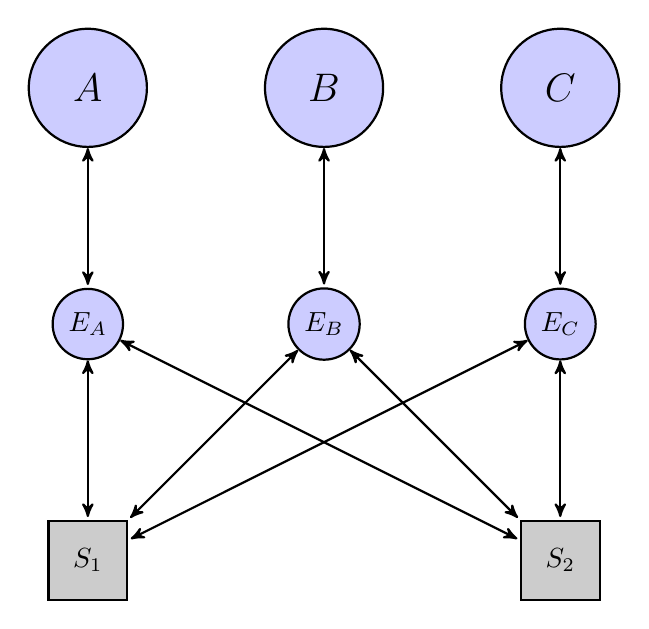
\begin{tikzpicture}[->,>=stealth',shorten >=1pt,auto,node distance=3cm,thick,
  main node/.style={circle,fill=blue!20,draw,font=\sffamily\Large\bfseries,
                   minimum size=15mm},
  switch node/.style={rectangle,draw,fill=black!20,minimum size=10mm},
  end node/.style={circle,draw,fill=blue!20,minimum size=8mm}]

  \node[main node] (A)               {$A$};
  \node[main node] (B) [right of=A]  {$B$};
  \node[main node] (C) [right of=B]  {$C$};

  \node[end node] (EA) [below of=A]   {$E_A$};
  \node[end node] (EB) [right of=EA]  {$E_B$};
  \node[end node] (EC) [right of=EB]  {$E_C$};

  \node[switch node] (S1) [below of=EA] {$S_1$};
  \node[switch node] (S2) [below of=EC] {$S_2$};

  % node to endpoints
  \draw[<->, thick] (A) to (EA);
  \draw[<->, thick] (B) to (EB);
  \draw[<->, thick] (C) to (EC);

  % endpoints to switches
  \draw[<->, thick] (EA) to (S1);
  \draw[<->, thick] (EA) to (S2);

  \draw[<->, thick] (EB) to (S1);
  \draw[<->, thick] (EB) to (S2);

  \draw[<->, thick] (EC) to (S1);
  \draw[<->, thick] (EC) to (S2);

\end{tikzpicture}
\caption{A switched ethernet network for 3 nodes and 2 switches}
\label{fig:swether-diagram}
\end{figure}

The network operates as follows. A node, say $A$, wants to broadcast a
message. It sends a message to an endpoint node $E_A$ that handles the
broadcast to each of the 2 switches $S_1$ and $S_2$. When a switch receives a
message it relays it to all the other endpoints on the network. The endpoints
are responsible for sorting out which message to eventually deliver to the
node. For simplicity we describe a network where endpoints deliver all
messages they receive from switches to their corresponding node.

To specify a network in LIMA we declare a function \y{mkSWEther} that takes as
parameters a number of nodes and a number of switches and returns a list of channel
input/output pairs. The channels are meant to be attached to user specified
nodes in a specific order. Internally, \y{mkSWEther} builds the endpoints and
switches as nodes and builds all the channels in between as well as those
pointing in and out of the network which will be returned.

Figure~\ref{fig:swether-internal-chans} shows how the internal channels are
built. There is a unidirectional channel for each switch and each endpoint and
each other endpoint. They are stored in a particular order for ease of use in
attaching them to switches and endpoints.

\begin{figure}
\begin{lima}
-- generate the internal channels: [ [ (in_k_j, [out_1, ...]) ] ]
-- where in_k_j goes from endpoint j to switch k and out_1 .. out_{n-1} go
-- from switch k to the other endpoints (but not the j-th).
internalChans <-
  forM rm # \k ->       -- loop over switches
    forM rn # \j -> do  -- loop over endpoints
      in_k_j <- channel (printf "in_s%d_e%d" k j) typ
      let mkOChan i = do c <- channel (printf "out_s%v_e%v_e%v" k j i) typ
                         return (i,c)
      outs <- mapM mkOChan (bar j)
      return (in_k_j, outs)
\end{lima}
\caption{Declaration of internal channels}
\label{fig:swether-internal-chans}
\end{figure}

The switches are built from atoms having $n$ handler sub-atoms. Each handler
listens to a particular incoming channel (from one of the endpoints) and
whenever it sees a message there it broadcasts it out to all the other
endpoints. The declaration of switches is seen in Figure~\ref{fig:swether-switches}.

\begin{figure}
\begin{lima}
-- generate the switches:
-- each one listes on each incoming chan and broadcast to all outgoing chans
forM_ rm # \k ->
  atom (printf "sw%v" k) # do
    let myChans = internalChans !! k  -- :: [ (in_k_j, outs) ]_j
    forM_ rn # \j -> do
      let (myIn, myOuts) = myChans !! j
      atom (printf "handler_%v_%v" k j) # do
        cond # fullChannel (snd myIn)
        v <- readChannel (snd myIn)
        mapM_ ((`writeChannel` (v :: E Typ)) . fst . snd) myOuts
\end{lima}
\caption{Declaration of switches}
\label{fig:swether-switches}
\end{figure}

The endpoints are mostly similar to the switches: they listen to the channel
coming from the corresponding node and broadcast and received message to the
switches. However, in the opposite direction we have a problem. Each endpoint
must also listen to all the switches and decide what to do with the messages.
Listening is not a problem, we simply declare sub-atoms for each incoming
switch channel and set them up to listen to the correct channel. But now we
need these sub-atoms to write each message they receive to the one outgoing
channel that points to the corresponding node. This is a problem because it
means we have multiple atoms writing to the same channel. This is not allowed
in LIMA by design. Instead we must buffer the sending of messages to the node.
In our case-study implementation we chose to buffer messages using a FIFO
queue of fixed length.

\subsection{Synchronous Fault-Tolerant OM(1) Systems}
\label{ssec:synchronous-om1}

\subsubsection{Informal Model}
Our first case study is is a system that implements one of the ``Oral Messages''
algorithms. These are synchronous, distributed, and fault-tolerant systems that
solve the Byzantine Generals Problem~\cite{Lamport-OM}. The family of systems
that implement $\OM{m}$ have different numbers of communicating nodes and
offer varying levels of fault tolerance. We've chosen to focus our attention
on systems that implement the specific algorithm $\OMH{1}$, ``Hybrid Oral
Messages with 1 Round''.  In this algorithm, $n$ nodes communicate in order to
reach agreement on a valid course of action (or equivalent information). This
is done in the presence of \emph{at most 1} faulty node, whose communications
and behavior are assumed to be completely unconstrained (``Byzantine''). The
difference between \OM(1) and \OMH(1) lies in the details of how certain types
of faulty messages are treated. \OMH(1) can be viewed as an extension of
\OM(1) which tolerates a broader set of fault patterns.

Figure~\ref{fig:om1} depicts the communication pattern for \OM{1} (and also
\OMH(1)). Each of the $n$ nodes in the system represents a (Byzantine)
General. In this formulation, the center node is the commanding general, while
the $n-1$ outer generals are the lieutenants. The algorithm starts with the
commanding general sending each lieutenant the same message $v$. Upon receipt
of the commander's message, each lieutenant in turn sends the message received
to each of the other lieutenants.  Once a lieutenant has received all $n-1$
expected messages, a majority vote is taken among the $n$ messages and the
lieutenant declares its output (course of action) to be whichever message is
in the majority.

\begin{figure}[ht]
\centering
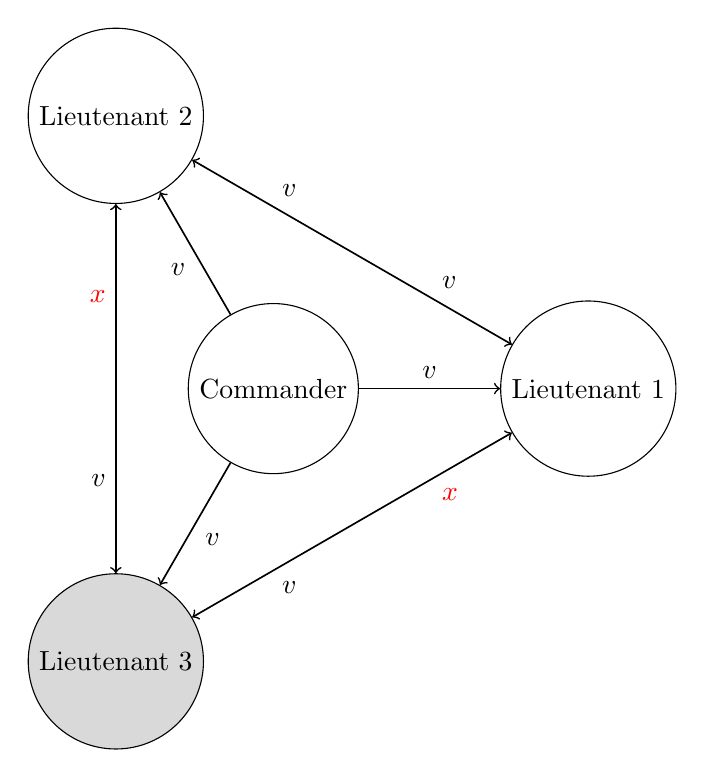
\begin{tikzpicture}[
ell/.style={x radius=1, y radius=0.5, draw, shape=circle},
arr/.style={semithick}]
\node[ell] (c)  at (0,0)   {Commander};
\node[ell] (l1) at (0:4)   {Lieutenant 1};
\node[ell] (l2) at (120:4) {Lieutenant 2};
\node[ell] (l3) [fill=gray!30] at (240:4) {Lieutenant 3};
%
\draw[->, arr] (c) -- node[auto] {$v$} (l1);
\draw[->, arr] (c) -- node[auto] {$v$} (l2);
\draw[->, arr] (c) -- node[auto] {$v$} (l3);
\draw[<->, arr] (l1) -- node[auto,swap,near start] {$v$}
                        node[auto,swap,near end] {$v$} (l2);
\draw[<->, arr] (l1) -- node[auto,near start,color=red] {$x$}
                        node[auto,near end] {$v$} (l3);
\draw[<->, arr] (l2) -- node[auto,swap,near start,color=red] {$x$}
                        node[auto,swap,near end] {$v$} (l3);
\end{tikzpicture}
\caption{\OMH{1} Four generals, one traitor}
\label{fig:om1}
\end{figure}

For a fault model we follow~\cite{Rushby-OM1} and assume that nodes are the
only source of faults. Moreover, node faults are assumed to be either
\emph{manifest}, \emph{symmetric}, or \emph{byzantine}. A fault is called manifest if
it is detectable by the non-faulty nodes; for example a node that sends to
another node a message that explicitly indicates there is a fault. On the
other hand, a fault is called symmetric if its presence is not necessarily
detectable as a fault to the other components; for example a node which sends
wrong messages, as opposed to invalid or missing messages.

Given a formal model of \OMH{1}, the standard target for verification is
\emph{validity} and \emph{agreement}. If we let $l_i$ denote the output for
lieutenant $i$ (where $1 \le i \le n-1$), then validity states:
%
\begin{equation}
    \forall \,i. \quad l_i = v
\end{equation}
%
whereas agreement states:
%
\begin{equation}
    \forall \,i, j. \quad l_i = l_j
\end{equation}
%
where $i,j$ range over the non-faulty nodes.

It is a classical result that \OM{1} can tolerate at most 1 (byzantine) faulty
node as long as there are at least 4 nodes in total. By adding additional
communication rounds, \OM{1} can be extended to an algorithm \OM{m} which
tolerates at most $m$ faults. On the other hand it is known that any system
which tolerates $m$ byzantine faults must involve at least $3m+1$ nodes.

In the results above there are several assumptions made regarding the
underlying computational platform which aren't obvious from the informal
description, but become so when one considers formally modelling it. To make
as many assumptions as possible explicit, we require:
\begin{enumerate}
    \item every message sent by a node is received successfully by the
        addressed node,
    \item when a node receives a message it may determine who sent it,
    \item each node can detect the absence of a message.
\end{enumerate}
These are the assumptions made by Lamport in his constructed solution for
$\OM{m}$ and the corresponding impossibility result (see
\cite{Lamport-OM}~\S2). It follows that a system implementing $\OM{1}$ must
transition synchronously. In particular, in an asynchronous system there is no
general method for detecting when a message is absent.

%% In Section~\ref{sssec:case-om1-sal} we present a formal model of $\OM{1}$ that
%% is the result of translating our ADSL specification to the transition system
%% language of SAL.

\subsubsection{ADSL Specification}

We now describe our implementation of Oral Messages in the ADSL. While we have specified
and verified the extension, \OMH(1) in the ADSL, we elide for simplicity the
differences between \OMH(1) and \OM(1) and just present \OM(1) here.

Our ADSL implementation of \OM(1) makes heavy use of the facilities of the
host language, Haskell. Indeed, the main part of the definition of the system
is given in just a few lines thanks to the use of parameterization.

\begin{figure}
\begin{lima}
om1 :: Atom ()
om1 = do
  -- setup channels for communication between source, relays, and receivers
  s2rs <- mapM newChannel ["s2r" ++ show i | i <- relaySet]
  r2rs <- mapM (mapM newChannel) [["r2r" ++ show i ++ show j | j <- recvSet]
                                                             | i <- relaySet]
  -- declare the set of vote variables that receivers will populate
  votes <- mapM msgVar ["vote" ++ show j | j <- recvSet]

  -- declare source node
  source (map fst s2rs)

  -- declare relay nodes
  forM_ relaySet 3 \idt ->
    relay ident (snd (s2rs !! idt))
                (map fst (r2rs !! idt))

  -- declare receiver nodes
  dones <- forM recvSet # \idt ->
    recv idt [snd ((r2rs !! i) !! idt) | i <- relaySet] (votes !! idt)

  -- state the "agreement" property
  let votesEqual (v,w) = value v ==. value w
  assert "agreement" # imply (and_ (map value dones))
                             (all_ votesEqual
                                   [(v,w) | v <- votes, w <- votes])

  -- state the "validity" property
  let voteGood v = value v ==. goodMsg
  assert "validity" # imply (and_ (map value dones)) (all_ voteGood votes)
\end{lima}
\caption{Setting up \OM(1)}
\label{fig:om1-setup}
\end{figure}

In this specification we refer to the Commander as the ``source'' and the
Lieutenants are unrolled into two sets: ``relays'' and ``receivers''. Here,
the source broadcasts to the relays which, in turn, broadcast to the
receivers which proceed with their vote. The code of Figure~\ref{fig:om1-setup} shows first channels being setup for communication, then
the source is declared by calling a function which we define shortly. The
relays and receivers are also declared by calling functions provided different
parameters.

For example, Figure~\ref{fig:om1-relay} shows the function definition for a
generic relay.

\begin{figure}
\begin{lima}
recv :: Int           -- ^ receiver id
     -> [ChanOutput]  -- ^ channels from relays
     -> V MsgType     -- ^ vote variable
     -> Atom (V Bool)
relay idt inC outCs = atom ("relay" ++ idt) # do
  -- declare local variables
  done <- bool "done" False
  msg  <- msgVar ("relay_msg" ++ idt)

  -- activation condition:
  --   we haven't stored a value yet and there is a message waiting
  --   on the channel 'inC'
  cond # isMissing msg &&. fullChannel inC

  -- behavior
  m <- readChannel inC
  msg  <== m
  done <== true
  forM_ outCs # \c -> writeChannel c m
\end{lima}
\caption{Function for declaring a generic relay}
\label{fig:om1-relay}
\end{figure}

The \y{relay} function takes an identifier, an incoming channel (for
receiving) and a list of channel outputs (for broadcasting). Recall that the
\y{cond} primitive acts as a guard on the atomic action to be taken in the
last 4 lines of the definition. In those last lines, the relay reads a message
from the incoming channel, stores it in a local variable, sets its \y{done}
flag, and then writes that message out on each of the outgoing channels it has.

The definition of \y{recv} is similar, except that each receiver possibly makes two
atomic actions through the declaration of two sub-atoms. The first sub-atom
listens for messages from the relays and fills a buffer as they arrive. The
second sub-atom is enabled only when the buffer is full and it computes a
majority vote on the buffer and stores the result in its \y{vote} variable
argument.

The majority vote computation is specified using the ``Fast Majority Vote''
algorithm due to Boyer and Moore \cite{mjrty}. This algorithm requires only a
single pass over the vote buffer. This is accomplished in our DSL using a
right fold operation as seen in Figure~\ref{fig:majority-vote}. A buffer value
and a counter are maintained during the pass. When the next element in the
buffer equals the currently maintained value, the counter is increased. If the
next element is different and the counter is zero, then the maintained value
is replaced, else the counter is decreased. In this way, at the end of the
pass, if there is a majority, it will be equal to the value maintained. It is worth
pointing out here that it is precisely this aspect, the level of detail in
implementing the majority vote, that sets our model of \OM(1) apart from
previous models.

\begin{figure}
\begin{lima}
computeVote :: [E MsgType] -> E MsgType
computeVote = fst . foldr iter (missingMsgValueE, 0)
  where
    iter x (y, c) = ( mux (x ==. y) onTrue1 onFalse1
                    , mux (x ==. y) onTrue2 onFalse2)
      where
        onTrue1       = y
        onTrue2       = c + 1
        onFalse1      = mux (c ==. 0) x y
        onFalse2      = mux (c ==. 0) 1 (c - 1)
\end{lima}
\caption{Fast Majority Vote in LIMA}
\label{fig:majority-vote}
\end{figure}

Finally, we have the system properties declared at the end of \y{om1} using
assertions. Both agreement and validity are predicated on the receivers being
done and the values in the list of vote variables.

\subsubsection{Generated Model}\label{sssec:om1-sally-model}

The formal model generated for \OM(1) by LIMA is quite large. Whereas the LIMA
specification file is only 5632 bytes, the Sally model LIMA generates for it
is 110,581 bytes. The generated model has 65 state variables, 12 input
variables, and 16 transitions in total. As an example of what the Sally model
looks like, consider the translation of the ``agreement'' property. Figure~\ref{fig:sally-query} shows the corresponding Sally query. The terms in the
query are rendered in $A$-normal form \cite{Sabry-Felleisen} to get maximum
benefit from sharing sub-terms.

\begin{figure}
\begin{sally}
(query
 om1_transition_system
 (let
  ((temp!0 true)
   (temp!1 om1!vote_2)
   (temp!2 om1!vote_1)
   (temp!3 (= temp!1 temp!2))
   (temp!4 om1!vote_0)
   (temp!5 (= temp!1 temp!4))
   (temp!6 (= temp!2 temp!1))
   (temp!7 (= temp!2 temp!4))
   (temp!8 (= temp!4 temp!1))
   (temp!9 (= temp!4 temp!2))
   (temp!10 (and temp!3 temp!5 temp!6 temp!7 temp!8 temp!9))
   (temp!11 (not temp!10))
   (temp!12 om1!recv_2!done)
   (temp!13 om1!recv_1!done)
   (temp!14 om1!recv_0!done)
   (temp!15 (and temp!11 temp!12 temp!13 temp!14))
   (temp!16 (not temp!15)))
  (not temp!15)))
\end{sally}
\caption{A Sally query rendered in $A$-normal form}
\label{fig:sally-query}
\end{figure}

Some verification of these models can be done automatically, without any
further work. For example, if we reduce \OM(1) system above so that it has
only 2 relays and 2 receivers, then the Sally model checker can automatically
verify that both agreement and validity hold in just over 11 minutes. With the
hybrid fault model assumption made, this is still a fairly non-trivial
verification and it is a highly non-trivial one for the model checker to
decide.

\subsection{Asynchronous  Airbus A320 Autobrake System}
\label{airbuscs}

\subsubsection{Informal Description}

The third  case-study is based on the runway excursion of an Airbus 320, occurring on
an Ibiza Airbus on 21st of May, 1998.  The full details of and the root cause
analysis are detailed in the incident report~\cite{a320ibiza}.  The excursion
resulted from a total loss of the braking system, due to the simultaneous
failure of  both channels of the Brake System Control Unit (BSCU) in conjunction
with a contamination within the braking system hydraulic system. From the ADSL
perspective, it is the failure of the software and BSCU architecture that is of
primary interest.

\begin{figure}
\begin{center}
\includegraphics[width=\textwidth]{figures/BSCU.pdf}
\caption{BSCU Function Schematic from~\cite{a320ibiza}.}
\label{fig:BSCU_schematic}
\end{center}
\end{figure}

In the A320 system as shown in Figure~\ref{fig:BSCU_schematic} from~\cite{a320ibiza}, the BSCU comprises two channels, with each channel incorporating command and monitor lanes.  The command lane provides the active
control path to the system, whereas the monitor lane checks and enforces that
the command lane is operating within the expected envelope of performance. On
the detection of the first failure, the monitoring lane indicates a failure, and
control is passed to the other channel.  All processing of the system is
executed using a quasi-synchronous computational model. That is to say,
processing of each channel is quasi-synchronous with respect to one another,
and the channels themselves are also quasi-synchronous.

In the Ibiza incident, the root cause of the loss of normal and alternative
braking systems, was the Byzantine induced failure of both BSCU channels. The
failure was due to the sampling of the auto-brake mode control input panel
buttons. The auto-brake panel comprise three buttons, \texttt{LO}, \texttt{MED} and \texttt{MAX} that can
be used to select the corresponding auto-braking mode.  Momentarily pushing the
\texttt{LO} button selects the \texttt{LO} auto-braking mode. Pressing \texttt{LO} again de-selects the
auto-braking function, whereas pressing the \texttt{MED} or \texttt{MAX} buttons  selects the
corresponding automatic braking  modes. The state of the selected mode is
communicated to the crew by indicators for each mode that are illuminated when
the corresponding mode is active.

In the Airbus implementation, the buttons were sampled periodically by software
every 25ms. Given the asynchronous composition of the system, each processor
samples the button state relative to its own operating time-line. This
implementation is vulnerable to short button presses that are too short ($< 25$ms)
and therefore not consistently perceived by all of the sampling units as shown in Figure~\ref{fig:push_button_sampling}.
(Additional inter-lane mode agreement logic, to mitigate Byzantine sampling is
not implemented in the system~\footnote{Given that the command and monitor lanes
  are configured to be a fault-set, best practice would have implemented ingress
  agreement logic to prevent a fault external to the pair from disrupting the
  paired agreement.}.) Hence, the system failure occurred when the command and
monitoring lanes of both channels fell into disagreement, following the momentary 
selection of the \texttt{LO} auto-brake mode. The \texttt{LO} selection was only detected by one
of the lanes of each channel, hence the command and monitor mode disagreement
detection logic was erroneously stimulated. In the excursion, the disagreement
occurred on both channels simultaneously. Given that the system mode logic was
also event driven, there was no path to recovery. Pressing \texttt{LO} would be subject
to the same Byzantine vulnerability, and even if not Byzantine, the
incrementally edge driven mode selection logic would not recover into a
consistent state.

\begin{figure}
\begin{center}
\includegraphics[width=\textwidth]{figures/newtrace.jpg}
\caption{Oscilloscope chart of pressing times of AUTO/BRK LO vs. acquisition times of COM/MON functions}
\label{fig:push_button_sampling}
\end{center}
\end{figure}

 The design errors represent a failure uncovered by the traditional design assurance
 framework.  Given the correct-by-construction synthesis focus, it is unlikely
 that our approach would allow such an implementation to be developed.  However,
 ensuring that the formal synthesis framework is sufficient to represent and
 explore such design vulnerabilities is a good test case for the ADSL formal
 tooling.  The A320 Airbus brake system offers a good case-study in asynchronous system design and verification. For example, the system also
 requires a protocol to manage the channel in control, and additional logic and
 protocols to that communication is healthy.  From the incident report these
 details of the Airbus protocol implementations in these areas are not
 available. From the description it appears that the channel-in-control logic
 utilizes an asymmetric power-on timeout to yield a first-up channel in
 control. This may also leave the system vulnerable to assumptions of BSCU
 power-on order, and transient recovery strategies.  The protocols may also be
 vulnerable to failures of the inter-lane and inter-channel communication lines.
  Utilizing the provisions within the LIMA\ workbench, the long-term goal
of this case-study is to support the systematic exploration of candidate
protocols and fault models; yielding a better understanding how protocol
and communication architecture related design decisions impact core-system
properties.
  \subsubsection{Formal Model}




The formal model  of the  Wheel Brake System closely follows the structure  of  Figures 2.
However, to simplify the logic, and to reduce the size of the model, the
three buttons of the brake control panel are abstracted into a single button
that selects between manual and auto-mode operation.  The channel in control
is also simplified from the temporal first-up raced based selection, to a  fixed-priority scheme, where a pre-configured preferred channel remains in control
until it is faulted. Although simpler this model is sufficient to explore and demonstrate the byzantine failure vulnerability of the original system. 

The formal model starts with a top-level wbs atom that is used
to host all the system subcomponents. At the top level, three channels
are also implemented, two to convey the button status to each of the lanes,
and a third to convey the button state to the lane observer processes, that are used to host the properties that re to be formally investigated.
The   implementation of the lanes leverages and illustrates DSL\ provisions for parameterized replication.
 Using a map as shown below,  each lane is instantiated using with an assigned boolean  priority;  as described above   this priority arbitrates which lane is on control when the system is in full-up operational mode (i.e. no faults present).

\begin{lima}
 -- Declare two lanes
  laneIns <- mapM mkLane [True, False]  -- high/low priority
\end{lima}

 The lane implementation comprises two clocked periodic processes, one each for the  command and monitor  functions, together with an  an initialization  atom. At every period, the command and monitor sample the input from the button and toggle status of a boolean  operational model variable \textit{cautoMode},  on the detection of a rising button edge.  At each period, the update status of the \textit{cautoMod}e variable is shared with the local lane monitor.
 The DSL\ extract for this logic is shown below.



\begin{lima}

   cautoMode <== mux ((value bs ==. Const True) &&.
                       (value prevbs ==. Const False))
                      (not_ (value cautoMode))
                      (value cautoMode)
    writeChannel ctoIn (value framecount)  -- send 'framecount' to observer
    writeChannel ctmIn (value cautoMode)
      
\end{lima}
  The principal periodic process of the monitor atom is symmetrical to the periodic command atom. However, the monitor logic is extended with additional agreement counting logic, to monitor the agreement of the local and  command lane exchanged   \emph{cautoMode}  status. If disagreement persists   for three periods, the  monitor channel yields control to the other lane, by signaling  agreement failure.  

\begin{lima}
atom "wait_x_side_autoMode" $ do
      cond $ fullChannel ctmOut
      v <- readChannel ctmOut
      xSideAutoMode <== v
      probeP "monitor.XsideAutoMode" (value xSideAutoMode)

 atom "mon_agreement" $ do
      agreementFailureCount <==
        mux (value mautoMode /=. value xSideAutoMode)
            (Const one + value agreementFailureCount)
            (Const zero)
      -- cond $ value mautoMode /=. value xSideAutoMode
      -- incr agreementFailureCount

    atom "mon_agreement_count" $ do
      cond $ value agreementFailureCount ==. Const three
      agreementFailure <== Const True

\end{lima}

The representation of the WBS\ model in the DSL\ is very compact with the core logic only requiring about 150 lines of code.
 When contrasted with the approximately 12,000
lines of sally code, which the LIMA\ synthesizes,  this is a significant reduction. It may be argued, that without such a DSL and the associated synthesis, the industrial viability of sally alone may be challenging.

  
 Properties of interest  are simply asserted within any of the atoms as illustrated below. However, it should be noted that the variables used within the assert statements need to be within the atom scope.
 To simply model construction and instrumentation, it is recommended that variables significant to system properties are sent to a top-level observer process, that can provide a central point of property specification.  


\begin{lima}
 atom "mon_agreement" $ do
   agreementFailureCount <=  =
        mux (value mautoMode /=. value xSideAutoMode)
            (Const one + value agreementFailureCount)
            (Const zero)
   assert (pName pp "my assert")(value agreementFailureCount <=. Const three)
\end{lima}

In the Airbus braking example, no physical faults were actually present. Hence, in our initial model, we also omit a  fault model. However, the DSL\ framework ensures that the full state of the asynchronous interaction of the sampling and channel in control logic, will be explored within the synthesized  sally model. Therefore, the workbench is anticipated to uncover the system Byzantine failure as part of the formal model analysis.

As part of future work, we intend to augment the fault model
of the intra-lane and inter-lane, communication channels, and use the DSL\
and workbench to explore how such failures can impact the assumed system
level invariants,
and safety properties. We also intend to re-introduce the first up   leader
election protocol, which selects the initial lane in control. One again,
we envisage that this will demonstrate how the DSL\ and formal analysis workbench will support the systematic exploration of how
potential faults, and start-up timing variations can disrupt and impact
system safety properties and assumptions.  \   


%% \subsubsection{Verification}

%% \begin{figure}
%% \begin{center}
%% \includegraphics[width=1.0\textwidth]{figures/WBS_results}
%% \caption{WBS Proofs, Lemmas, Scalability Results and Performance}
%% \label{fig:WBS_results}
%% \end{center}
%% \end{figure}

%% Figure \ref{fig:WBS_results} summarizes the k-inductive proofs of the two code listings \ref{lst:wbssal1} and \ref{lst:wbssal2} and the set of lemmas that need to first proved before subsequently proving the desired properties of WBS listed in section \ref{subsubsec:ADSL_WBS_SAL}. We then also provide the scalability results with respect how much \emph{depth ('k' in k-induction)} is required to prove the lemmas/properties and also show timing/performance in terms of wall clock time.

%% The properties \emph{disagree\_a, disagree\_b, channel\_a\_in\_control} for code listing \ref{lst:wbssal1} and properties \emph{disagree\_b, channel\_b\_in\_control,channel\_a\_or\_b\_in\_control} for code listing \ref{lst:wbssal2} has already been described in section \ref{subsubsec:ADSL_WBS_SAL}. Next we describe the individual lemmas:

%% \begin{enumerate}

%% \item \emph{clock\_invariant} in lines $325-344,399$ of code listing \ref{lst:wbssal1}: This is a lemma that proves 4 things: (i) time is always non-negative or has value -1 indicating mutex (for exclusive operation on the calendar) (ii) time progresses montonously increasing i.e. the calendar processes each temporal event such that the next processed time is never less than the previous time (iii) mutexes on the calendar is processed atomically whereby if any task has the same value of -1 implies the the two tasks are identical and (iv) time is processed systematically so that all task clocks  for $com1$, $mon1$, $com2$ and $mon2$ are within the same period and their phase differences between the task clocks are properly advanced. \emph{Comment: This lemma is expected to be automatically generated from the ADSL}

%% \item \emph{auto\_mode\_invariant} in lines $354-360,401$ of code listing \ref{lst:wbssal1}: Ensures the \emph{initialization} of $com1$, $mon1$, $com2$ and $mon2$ i.e. com and mon across both channels a and b are properly initialized if the $button$ has not been pressed. \emph{This lemma is expected to be automatically generated from the ADSL} 

%% \item \emph{seen\_rising\_edge} in lines $366,402$ of code listing \ref{lst:wbssal1}: This lemma proves that if time has progressed greater than \emph{twice} the sampling period of $com1$, $mon1$, $com2$ and $mon2$, then the \emph{rising edge} of the push button of being pressed is guaranteed be detected by all of nodes $com1$, $mon1$, $com2$ and $mon2$. Alternatively if time is -1 (mutex) or had progressed to be less than the sampling period of $com1$, $mon1$, $com2$ and $mon2$, then the \emph{rising edge} of the push button of being pressed is guaranteed to NOT be detected by any of nodes $com1$, $mon1$, $com2$ and $mon2$. \emph{This lemma is expected to be manually specified within the ADSL} 

%% \item \emph{button\_invariant} in lines $347-351,400$ of code listing \ref{lst:wbssal1}: Proves that the button state variables are properly initialized. \emph{This lemma is expected to be automatically generated from the ADSL} 

%% \item \emph{cs} in lines $364,403$ of code listing \ref{lst:wbssal1}: This lemma proves that if time has progressed greater than \emph{twice} the sampling period of $com1$, $mon1$, $com2$ and $mon2$, then $com1$ mode selection must match $mon1$ and also $com2$ mode selection must match $mon2$ as sufficient time has elapsed for the two channels to both see the push button being pressed and hence \emph{seen\_rising\_edge} being detected. \emph{This lemma is expected to be manually specified within the ADSL} 

%% \item \emph{fixed\_fault\_mon\_a\_fail} in lines $522$ of code listing \ref{lst:wbssal2}: Directly based on the fault hypothesis. \emph{This lemma is expected to be automatically generated from the ADSL} 

%% \item \emph{cs\_b} in lines $456,512$ of code listing \ref{lst:wbssal2}: This lemma proves that if time has progressed greater than \emph{twice} the sampling period of $com2$ and $mon2$, then $com2$ mode selection must match $mon2$ as sufficient time has elapsed for the two channels to both see the push button being pressed and hence \emph{seen\_rising\_edge} being detected. \emph{This lemma is expected to be manually specified within the ADSL} 

%% \item \emph{button\_phase\_invariant} in lines $428-436,505$ of code listing \ref{lst:wbssal2}: The lemma ensures that time is processed systematically so that all task clocks  for $com1$, $mon1$, $com2$ and $mon2$ are within the same period and their phase differences between the task clocks are properly advanced and simultaneously ensuring these are done before the \emph{button} $period$ which is at a much slower rate. \emph{Comment: This lemma is expected to be automatically generated from the ADSL}

%% \end{enumerate}

%% As seen above, except for 3 lemmas (\emph{seen\_rising\_edge,cs,cs\_b}) which have to manually generated from ADSL, the rest of them can be automatically generated. Further the methodology to automatically deduce the \emph{depth} for k-induction (3rd column in figure \ref{fig:WBS_results}) must be investigated. Finally the dependencies or order of proving lemmas before proving the properties (listed in 2nd column in figure \ref{fig:WBS_results}) must also be investigated. \emph{These three issues listed must be resolved before AFFIRM workbench can guarantee that the necessary lemmas and k-induction proof of properties can automatically be synthesized}.  

%% \begin{figure}
%% \begin{center}
%% \includegraphics[width=1.0\textwidth]{figures/WBS_results}
%% \caption{WBS Proofs, Lemmas, Scalability Results and Performance}
%% \label{fig:WBS_results}
%% \end{center}
%% \end{figure}

%% Figure \ref{fig:WBS_results} summarizes the k-inductive proofs of the two code listings \ref{lst:wbssal1} and \ref{lst:wbssal2} and the set of lemmas that need to first proved before subsequently proving the desired properties of WBS listed in section \ref{subsubsec:ADSL_WBS_SAL}. We then also provide the scalability results with respect how much \emph{depth ('k' in k-induction)} is required to prove the lemmas/properties and also show timing/performance in terms of wall clock time.

%% The properties \emph{disagree\_a, disagree\_b, channel\_a\_in\_control} for code listing \ref{lst:wbssal1} and properties \emph{disagree\_b, channel\_b\_in\_control,channel\_a\_or\_b\_in\_control} for code listing \ref{lst:wbssal2} has already been described in section \ref{subsubsec:ADSL_WBS_SAL}. Next we describe the individual lemmas:

%% \begin{enumerate}

%% \item \emph{clock\_invariant} in lines $325-344,399$ of code listing \ref{lst:wbssal1}: This is a lemma that proves 4 things: (i) time is always non-negative or has value -1 indicating mutex (for exclusive operation on the calendar) (ii) time progresses montonously increasing i.e. the calendar processes each temporal event such that the next processed time is never less than the previous time (iii) mutexes on the calendar is processed atomically whereby if any task has the same value of -1 implies the the two tasks are identical and (iv) time is processed systematically so that all task clocks  for $com1$, $mon1$, $com2$ and $mon2$ are within the same period and their phase differences between the task clocks are properly advanced. \emph{Comment: This lemma is expected to be automatically generated from the ADSL}

%% \item \emph{auto\_mode\_invariant} in lines $354-360,401$ of code listing \ref{lst:wbssal1}: Ensures the \emph{initialization} of $com1$, $mon1$, $com2$ and $mon2$ i.e. com and mon across both channels a and b are properly initialized if the $button$ has not been pressed. \emph{This lemma is expected to be automatically generated from the ADSL} 

%% \item \emph{seen\_rising\_edge} in lines $366,402$ of code listing \ref{lst:wbssal1}: This lemma proves that if time has progressed greater than \emph{twice} the sampling period of $com1$, $mon1$, $com2$ and $mon2$, then the \emph{rising edge} of the push button of being pressed is guaranteed be detected by all of nodes $com1$, $mon1$, $com2$ and $mon2$. Alternatively if time is -1 (mutex) or had progressed to be less than the sampling period of $com1$, $mon1$, $com2$ and $mon2$, then the \emph{rising edge} of the push button of being pressed is guaranteed to NOT be detected by any of nodes $com1$, $mon1$, $com2$ and $mon2$. \emph{This lemma is expected to be manually specified within the ADSL} 

%% \item \emph{button\_invariant} in lines $347-351,400$ of code listing \ref{lst:wbssal1}: Proves that the button state variables are properly initialized. \emph{This lemma is expected to be automatically generated from the ADSL} 

%% \item \emph{cs} in lines $364,403$ of code listing \ref{lst:wbssal1}: This lemma proves that if time has progressed greater than \emph{twice} the sampling period of $com1$, $mon1$, $com2$ and $mon2$, then $com1$ mode selection must match $mon1$ and also $com2$ mode selection must match $mon2$ as sufficient time has elapsed for the two channels to both see the push button being pressed and hence \emph{seen\_rising\_edge} being detected. \emph{This lemma is expected to be manually specified within the ADSL} 

%% \item \emph{fixed\_fault\_mon\_a\_fail} in lines $522$ of code listing \ref{lst:wbssal2}: Directly based on the fault hypothesis. \emph{This lemma is expected to be automatically generated from the ADSL} 

%% \item \emph{cs\_b} in lines $456,512$ of code listing \ref{lst:wbssal2}: This lemma proves that if time has progressed greater than \emph{twice} the sampling period of $com2$ and $mon2$, then $com2$ mode selection must match $mon2$ as sufficient time has elapsed for the two channels to both see the push button being pressed and hence \emph{seen\_rising\_edge} being detected. \emph{This lemma is expected to be manually specified within the ADSL} 

%% \item \emph{button\_phase\_invariant} in lines $428-436,505$ of code listing \ref{lst:wbssal2}: The lemma ensures that time is processed systematically so that all task clocks  for $com1$, $mon1$, $com2$ and $mon2$ are within the same period and their phase differences between the task clocks are properly advanced and simultaneously ensuring these are done before the \emph{button} $period$ which is at a much slower rate. \emph{Comment: This lemma is expected to be automatically generated from the ADSL}

%% \end{enumerate}

%% As seen above, except for 3 lemmas (\emph{seen\_rising\_edge,cs,cs\_b}) which have to manually generated from ADSL, the rest of them can be automatically generated. Further the methodology to automatically deduce the \emph{depth} for k-induction (3rd column in figure \ref{fig:WBS_results}) must be investigated. Finally the dependencies or order of proving lemmas before proving the properties (listed in 2nd column in figure \ref{fig:WBS_results}) must also be investigated. \emph{These three issues listed must be resolved before AFFIRM workbench can guarantee that the necessary lemmas and k-induction proof of properties can automatically be synthesized}.  

%% \subsection{Time-Division, Multi-Access Protocol\ Start-up}\label{sec:tdma}


\subsubsection{Informal Description}

The case-study targets the transition from the asynchronous to synchronous operation. It is selected to ensure that the ADS\ It is useful to  
\subsubsection{Formal Model}


% ------------------------------------------------------------------------------
\section{Conclusions}
\label{sec:future-work}
We have laid out a vision in this technical report for an architectural domain
specific language and associated tools. Our work is heavily driven by
real-world case-studies, which we have covered in depth. We hope to convince
the reader that there is an industrial need for simplifying the specification
and verification of distributed fault-tolerant systems and for connecting
specifications to their implementations. We have described related work toward
this end, as well as our work in building the underlying constructs to support
a language and modeling framework. Much of our focus has been on the
specification and verification aspects, as we believe that formal proof is
necessary for tedious, high-consequence systems.

Although we have promising results and worked case-studies, the future work
associated with the research agenda involves significant engineering
work which we hope to address in coming years. This includes both developing the
modeling workbench itself as well as fleshing out more substantial case-studies.


\section*{Acknowledgments}
This work is supported by NASA contract \#NNL14AA08C. All findings are our own and do not necessarily reflect the opinions of NASA or the United States Government.
We particularly thank Wilfredo Torres-Pomales and Paul Miner at NASA Langley for their discussions, insights, and guidance. We thank Tom Hawkins, the original developer of the Atom language that we extend to produce LIMA.
Portions of this paper, and particularly Section~\ref{ssec:calendar}, are adapted from a conference paper~\cite{jones:nfm17}.

\section*{References}
\bibliographystyle{unsrt}
%\bibliographystyle{apalike}
\bibliography{bib}

\end{document}

